Cominciamo la seconda parte del corso, in questo momento vorremo dato qualunque segnale tempo discreto decomporlo in sinusoidi e vorremo capire quali cosinuosoidi possono fare da filtri per quel segnale e capire meglio cosa fa un sistema.

Inizialmente vediamo a che punto siamo arrivati e capiamo quali segnali abbiamo visto e come possiamo decomporli e ricomporli.

\begin{figure}[ht!]
    \centering
    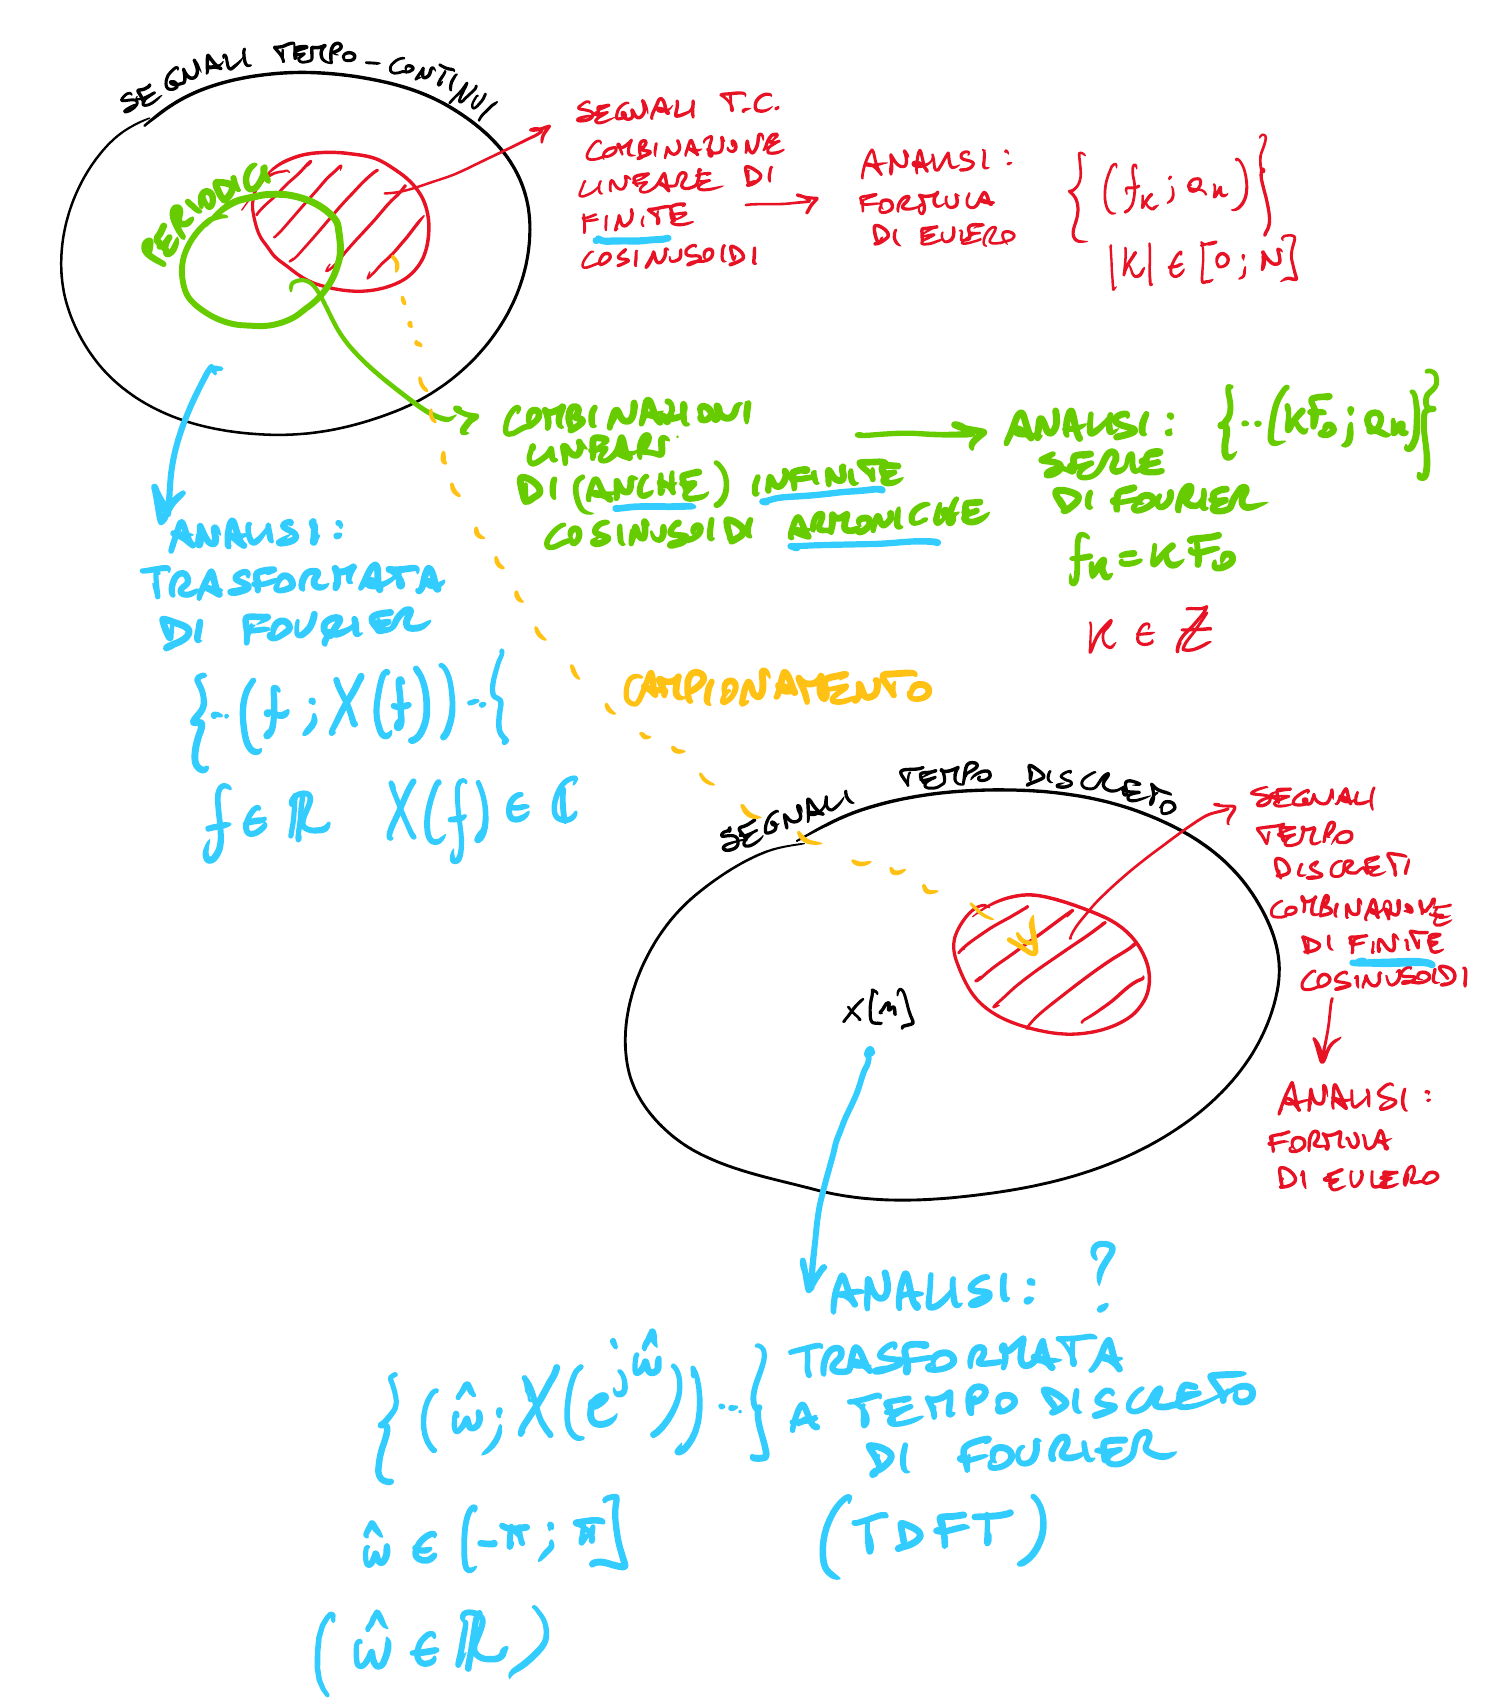
\includegraphics[scale=0.35]{immagini/lez17/segnali.jpg}
\end{figure}

\section{Trasformata a tempo discreto di Fourier (DTFT)}
Studiamo adesso la trasformata a tempo discreto di Fourier, la quale ci permettera' di scrivere lo spettro (fare l'analisi) di un qualunque segnale a tempo discreto.
Analisi:

\begin{equation}
    X(e^{j \hat{\omega}}) = \sum_{n = - \infty}^{+ \infty} x[n] e^{\textcolor{red}{-} j \hat{\omega} n}
\end{equation}

Notiamo inizialmente che questa formula e' molto simile alla risposta in frequenza tranne per un segno -.

Inoltre ricordando la definizione di prodotto scalare tra due segnali tempo discreti:

\[
    <x[n]; y[n]> = \sum_{n = - \infty}^{+ \infty} x[n] \cdot y^*[n]
\]

notiamo che i fasori discreti sono uguali al prodotto scalare tra $x[n]$ e $y^*[n] = e^{j \hat{\omega} n} $, in pratica possiamo riscrivere la DTFT come il prodotto scalare tra un segnale tempo discreto ed una base ortonormale: 
\[
    X(e^{j \hat{\omega}}) = <x[n]; e^{j \hat{\omega} n}>
\]

Inoltre ricordando la serie di Fourier per il tempo continuo, notiamo che c'e' un parallelismo, perche' anche in quel caso l'analisi di un segnale (fatta con un integrale) era uguale al prodotto scalare tra il segnale stesso ed una base ortonormale:

\[
    ak = \frac{1}{T_0} \int_0^{T_0} x(t) \cdot e^{-j 2\pi F_0 k t} dt = <x(t); e^{j 2\pi F_0 k t}>
\]

Formula di SINTESI:

\begin{equation}
    x[n] = \frac{1}{2\pi} \int_{-\pi}^{\pi} X(e^{j \hat{\omega}}) e^{j \hat{\omega} n } \phi \hat{\omega}
\end{equation}

Anche per quanto riguarda la forumla di sintesi notiamo il parallelismo con la sintesi della serie di Fourier per i segnali a tempo continuo:

\[
    x(t) = \sum_{k = - \infty}^{+ \infty} ak e ^{j 2\pi F_0 k t}
\]

Vediamo anche se consideriemo le frequenze come cambia la formula di Sintesi della DTFT:

\[\begin{split}
    \hat{\omega} &= 2\pi \hat{f} \\
    d \hat{\omega} &= 2\pi d \hat{f} \\
    &= 1 \int_{-\frac{1}{2}}^{\frac{1}{2}} X(e^{j 2\pi \hat{f}}) e^{j 2\pi \hat{f}} d \hat{f}
\end{split}\]

Elenchiamo adesso le proprieta' della DTFT.

\subsection{DTFT e' periodica di periodo $2\pi$}

Per verificare che sia vero proviamo a calcolare la DTFT in multipli di $2\pi$ per vedere se otteniamo lo stesso risultato, dove $h \in \mathbf{Z}$:

\[
    X(e^{j (\hat{\omega} + 2\pi h)}) = \sum_{n = - \infty}^{+ \infty} x[n] e^{-j n (\hat{\omega} + 2\pi h)} = \sum_{n = - \infty}^{+ \infty} x[n] e^{-j \hat{\omega} n} \cdot e^{-j n 2\pi h}
\]

A questo punto notiamo che il termine $e^{-j n 2\pi h}$ e' il numero 1, quindi abbiamo ottenuto esattamente la DTFT.

\subsection{La DTFT gode della proprieta' si simmetria coniugata se $x[n]$ e' reale}

Quello che significa questa proprieta' e':

\[
     X(e^{j \hat{\omega}}) =  X^*(e^{-j \hat{\omega}})
\]

Il corollario di questa proprieta' e' che la parte reale di $ X(e^{j \hat{\omega}})$, ovvero il modulo, e' una funzione pari, mentre la parte immaginaria di $ X(e^{j \hat{\omega}})$, la fase, e' una funzione dispari.

\subsection{La DTFT e' un operatore lineare}
Dati due coeficienti $\alpha, \beta \in \mathbf{R}$ se sappiamo che:

\[\begin{split}
    x_1[n] &\xrightarrow[]{\text{DTFT}} X_1(e^{j \hat{\omega}}) \\
    x_2[n] &\xrightarrow[]{\text{DTFT}} X_2(e^{j \hat{\omega}}) 
\end{split}\]

allora

\[
    \alpha x_1[n] + \beta x_2[n] x_1[n] \xrightarrow[]{\text{DTFT}} \alpha X_1(e^{j \hat{\omega}}) + \beta X_2(e^{j \hat{\omega}})
\]

\subsection{Se esiste la DTFT di $x[n]$, allora e' unica}
Dimostriamola per assurdo, dati due segnali li trasformiamo in una DTFT comune:

\[\begin{split}
    x_1[n] &\xrightarrow[]{\text{DTFT}} X(e^{j \hat{\omega}}) \\
    x_2[n] &\xrightarrow[]{\text{DTFT}} X(e^{j \hat{\omega}}) 
\end{split}\]

Ma se consideriamo un segnale che e' la differenza tra i due precedenti otteniamo ovviamente 0, in quanto, utilizzando la proprieta' di linearita' appena descritta la DTFT dei due e' uguale:

\[
    x[n] = x_1[n] - x_2[n] \xrightarrow[]{\text{DTFT}} X(e^{j \hat{\omega}})- X(e^{j \hat{\omega}}) = 0
\]

Ma questo vorrebbe dire che esiste un segnale la cui DTFT e' 0, ma questo puo' succedere solo se i due segnali sono uguali.

\subsection{Esempio 1}
Guardiamo ora lo spettro di alcuni segnali cosinusoidali.
Inizialmente consideriamo una delta traslata di $n_0$:

\begin{figure}[ht!]
    \centering
    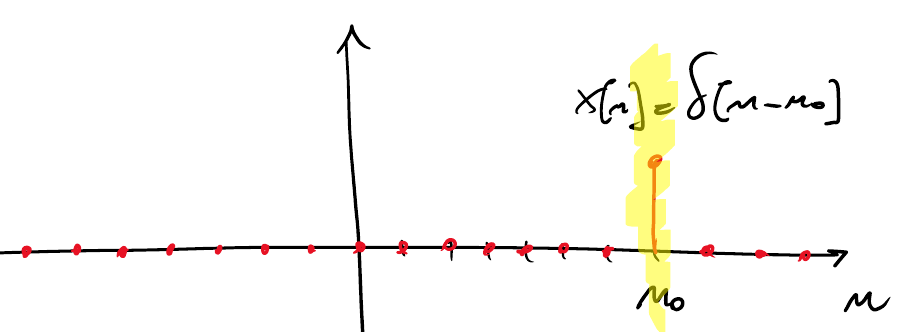
\includegraphics[scale=0.35]{immagini/lez17/esempio1.jpg}
\end{figure}

Per calcolare lo spettro applichiamo troviamo la DTFT del segnale applicando la definizione:

\[
    X(e^{j \hat{\omega}}) = \sum_{-\infty}^{+ \infty} \delta[n - n_0] e^{-j \hat{\omega} n}
\]

Ma sappiamo che la delta vale sempre zero tranne in $n_0$, di conseguenza la sommatoria si risolve in:

\[
    X(e^{j \hat{\omega}}) = e^{-j \hat{\omega} n_0}
\]

Tracciamo il grafico del modulo e della fase, il modulo e' costante ed e' 1 (ricordiamo che il modulo e' il numero intero che moltiplica l'esponenziale), mentre la fase e' uguale alla retta $y = -n_0 x$:

\begin{figure}[ht!]
    \centering
    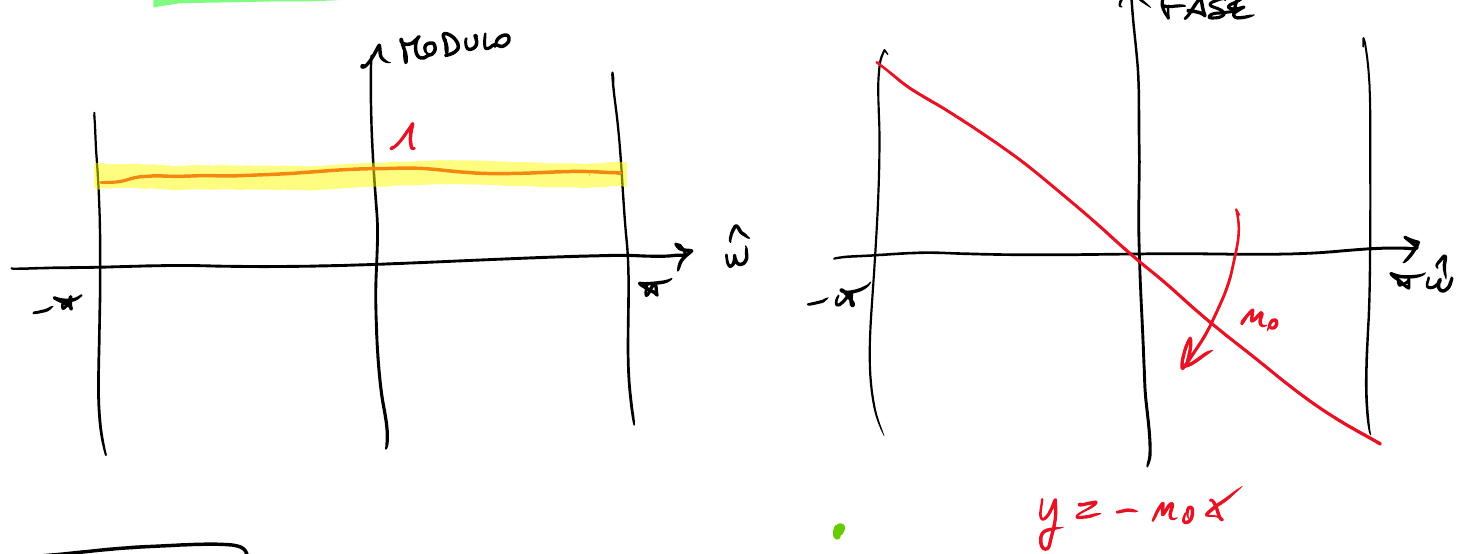
\includegraphics[scale=0.35]{immagini/lez17/moduloFaseEs1.jpg}
\end{figure}

\subsection{Esempio 2}
Come secondo esempio consideriamo il segnale esponenziale moltiplicato per il segnale calino:

\[
    x[n] = a^n \cdot u[n]
\]



\begin{figure}[ht!]
    \centering
    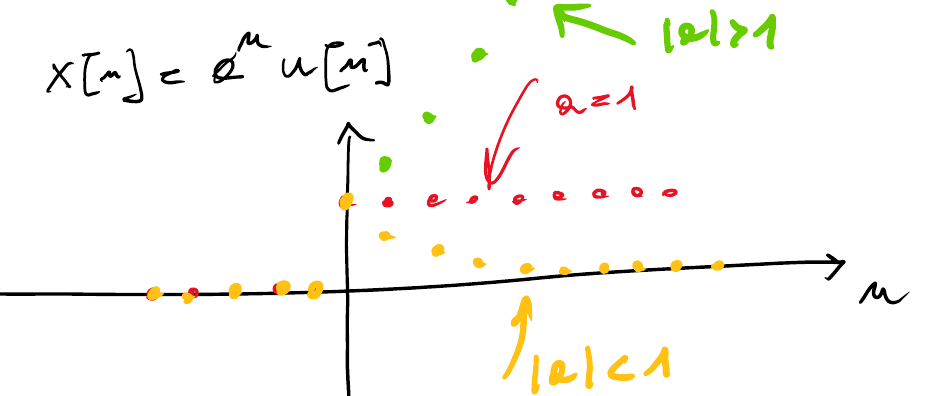
\includegraphics[scale=0.35]{immagini/lez17/esempio2.jpg}
\end{figure}

Come prima calcoliamo la DTFT del segnale applicando la formula:

\[
    DTFT\{ x[n] = a^n \cdot u[n] \} = \sum_{n = -\infty}^{+ \infty} a^n \cdot u[n] e^{-j \hat{\omega} n}
\]

Modifichiamo gli estremi della sommatoria dato che se $n<0$ la funzione non esiste, inoltre utilizziamo la sommatoria nota $\sum_{k=0}^{L-1}q^L = \frac{1-q^L}{1-q}$:

\[
    \sum_{n = 0}^{+\infty}(a e^{-j \hat{\omega}})^n = \lim_{N\to\infty}\frac{1 -(a e^{-j \hat{\omega}})^n}{a e^{-j \hat{\omega}}}
\]

Se $|a e^{-j \hat{\omega}}| < 1$ allora otteniamo $\frac{1}{1 - ae^{-j\hat{\omega}}}$

\section{Esempi con luce}
Vediamo un parallelismo tra l'analisi tramite DTFT di un segnale con la scomposizione di un fascio di luce bianca tramite un primsa e vediamo che decomponendo un segnale tramite la DTFT otteniamo lo spettro.

\begin{figure}[ht!]
    \centering
    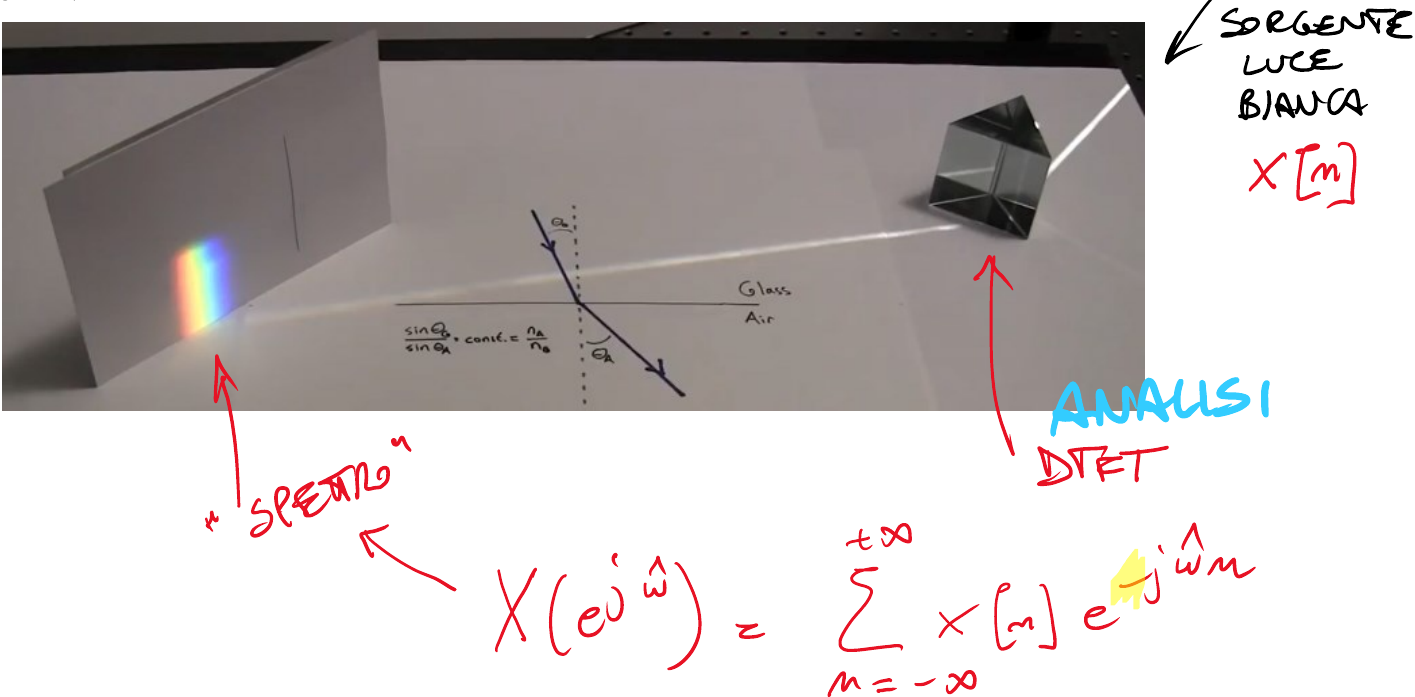
\includegraphics[scale=0.35]{immagini/lez18/sintesi.jpg}
\end{figure}

Quando invece vogliamo ricomporre lo spettro di un segnale utilizziamo la trasformata inversa IDTFT:

\begin{figure}[ht!]
    \centering
    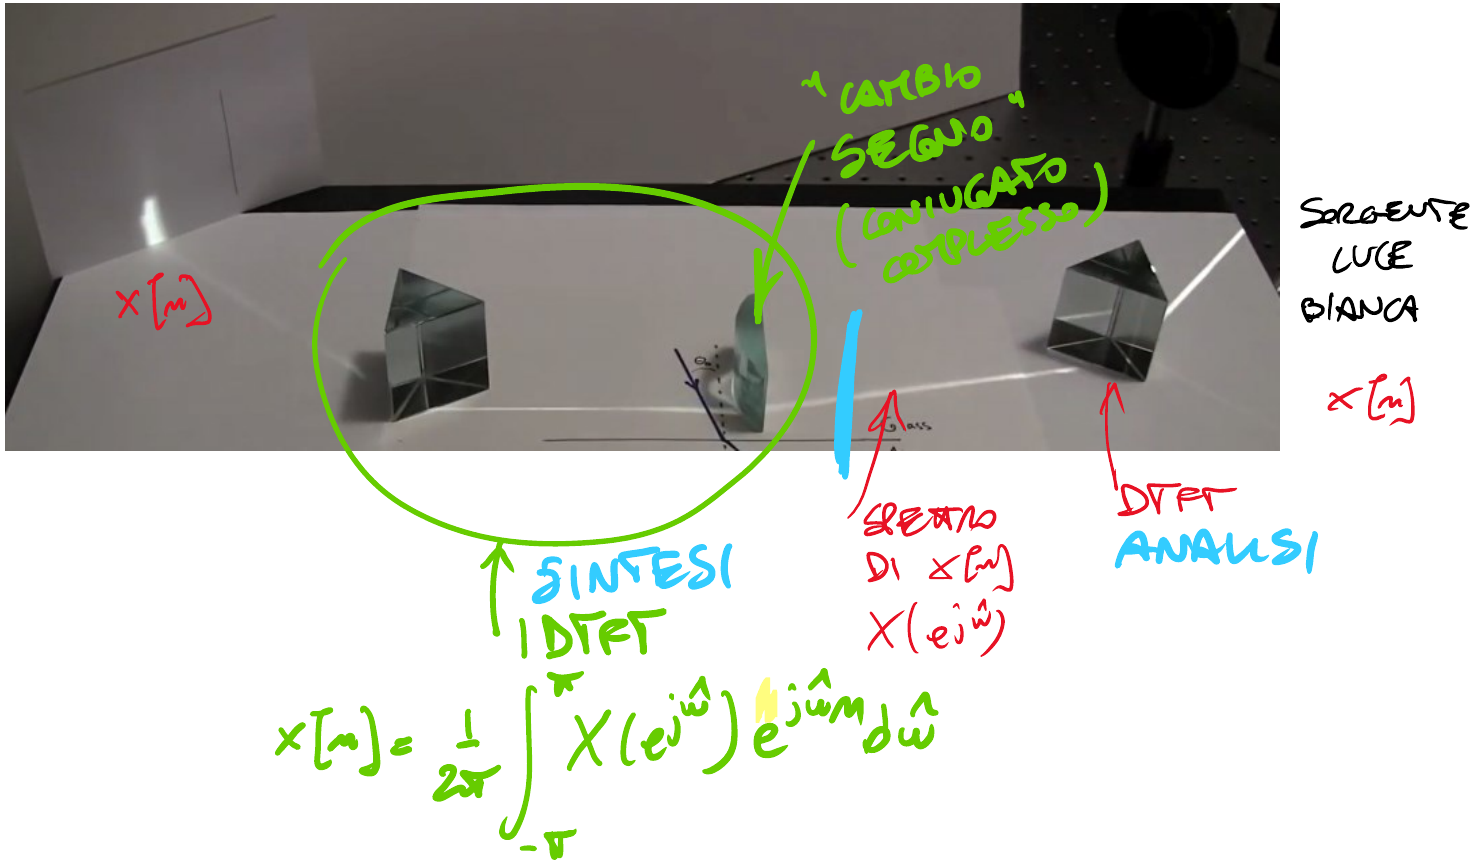
\includegraphics[scale=0.35]{immagini/lez18/analisiSintesi.jpg}
\end{figure}

La formula della IDTFT:

\begin{equation}
    x[n] = \frac{1}{2\pi} \int_{-\pi}^{\pi} X(e^{j \hat{\omega}}) e^{j \hat{\omega}n} d \hat{\omega}
\end{equation}

\section{Esempio}
Partiamo dal grafico del modulo e della fase di un segnale, e notiamo subito che assomiglia ad un filtro passa basso, di conseguenza le frequenze comprese tra $-\hat{w}_c$ e $\hat{w}_c$ passano, le altre vengono eliminate

\begin{figure}[ht!]
    \centering
    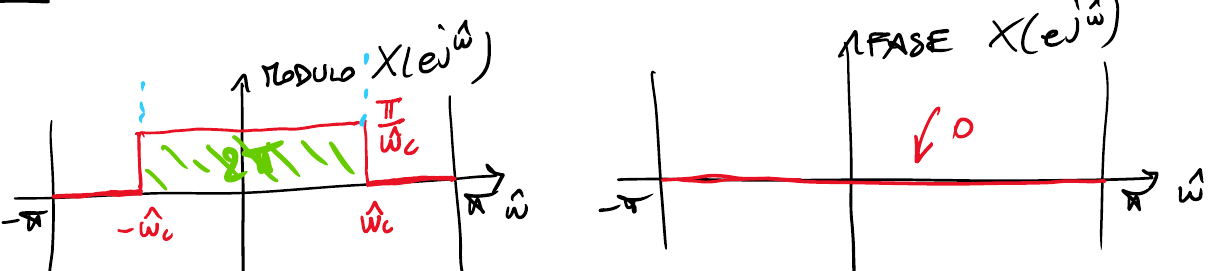
\includegraphics[scale=0.35]{immagini/lez18/esempio3ModuloFase.jpg}
\end{figure}

Utilizziamo la formula della IDTFT per ricostruire il segnale:

\[\begin{split}
    x[n] &= \frac{1}{2\pi} \int_{-\pi}^{\pi} \mbox{BOX}_{\hat{w}_c}(t) e^{j \hat{\omega}n} d \hat{\omega} = \frac{1}{2\pi} \int_{-\hat{w}_c}^{w_c} \frac{\pi}{\hat{w}_c} e^{j \hat{\omega}n} d \hat{\omega} \\
    &= \frac{1}{2 \hat{\omega}_c} [\frac{e^{j \hat{\omega} n}}{jn}]_{-\hat{\omega}}^{\hat{\omega}_c} = \frac{1}{2\hat{\omega}} \{ \frac{e^{j \hat{\omega}_c n}}{jn} - \frac{e^{-j \hat{\omega}_c n}}{jn} \} \\
    &= \frac{\sin \hat{\omega}_c n}{\hat{\omega}_ c} = sinc(\hat{\omega}_c n)
\end{split}\]

\begin{figure}[ht!]
    \centering
    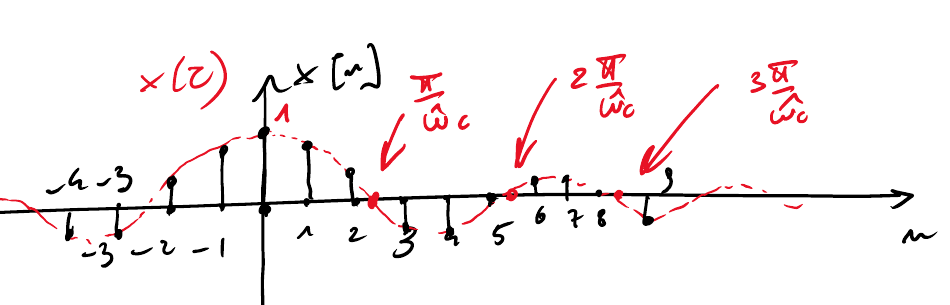
\includegraphics[scale=0.35]{immagini/lez18/casoGenerale.jpg}
\end{figure}

Quindi la ricostruzione di un filtro passa basso e' un sinc.

\medskip
\medskip
\medskip
\medskip
\medskip
\medskip
\medskip
\medskip
\medskip
\medskip
\medskip
\medskip
\medskip
\medskip
\medskip
\medskip
\medskip
\medskip
\medskip
\medskip
\medskip
\medskip
\medskip
\medskip
\medskip
\medskip
\medskip
\medskip
\medskip
\medskip
\medskip

Ora consideriamo dei casi particolari di questo filtro, inizialmente vediamo quando facciamo tendere $-\hat{w}_c$ e $\hat{w}_c$ a 0:

\begin{figure}[ht!]
    \centering
    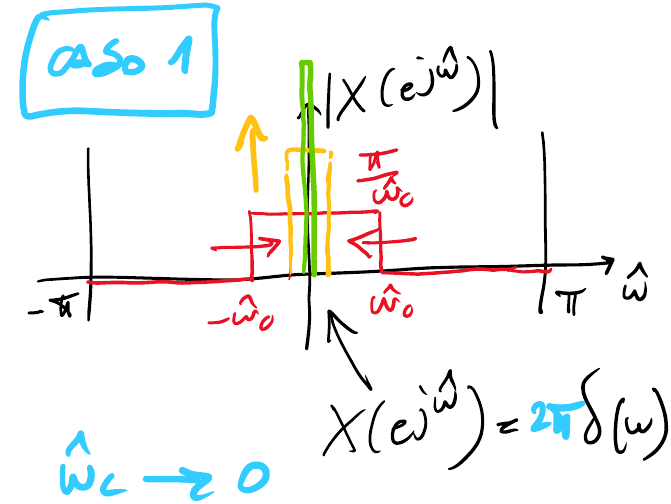
\includegraphics[scale=0.35]{immagini/lez18/casoParticolare1.jpg}
\end{figure}

Quello che succede e' che stringo il BOX e piu' lo stringo piu' l'altezza deve aumentare, ma l'area rimane uguale:

\begin{figure}[ht!]
    \centering
    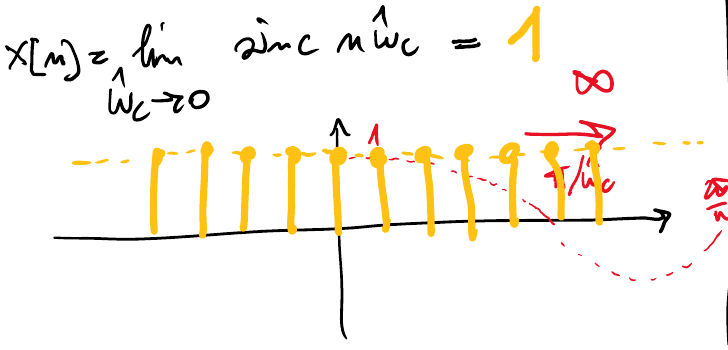
\includegraphics[scale=0.35]{immagini/lez18/estremoCaso1.jpg}
\end{figure}

Come secondo caso particolare invece vediamo cosa succede quando facciamo tendere $-\hat{w}_c$ e $\hat{w}_c$ a $\pi$, quello che succede e' che diminuisce l'altezza del BOX e diminuisce l'altezza.

\begin{figure}[ht!]
    \centering
    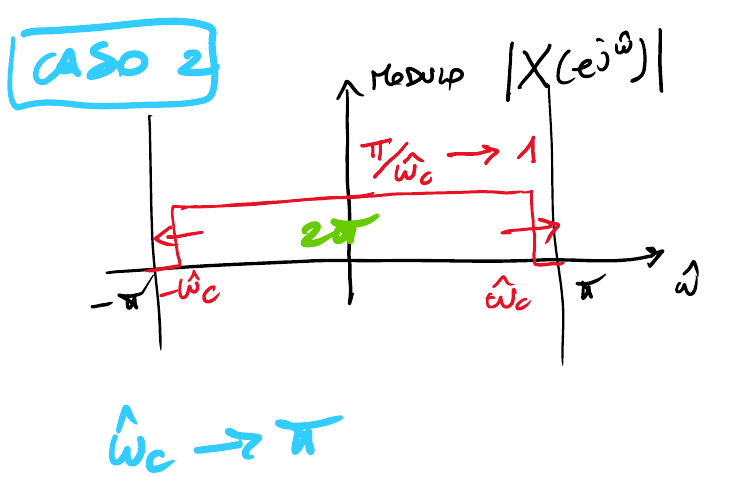
\includegraphics[scale=0.35]{immagini/lez18/casoParticolare2.jpg}
\end{figure}

Quello che otteniamo e' un sinc in cui sostituiamo $\hat{\omega}_c = \pi$, quindi e' una delta centrata in 0:

\begin{figure}[ht!]
    \centering
    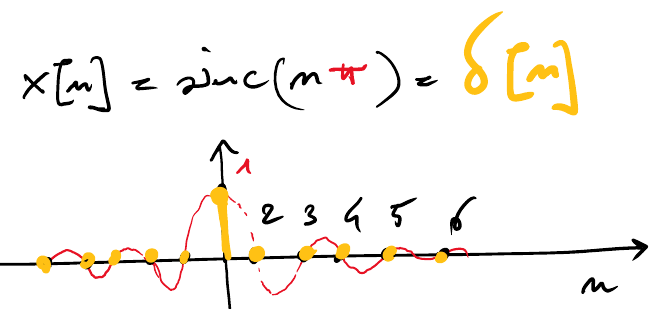
\includegraphics[scale=0.35]{immagini/lez18/estremoCaso2.jpg}
\end{figure}

\section{Delta di Dirac (funzione continua)}

E' una funzione generalizzata (o distribuzione), e' un'estensione al limite di una funzione che possiamo usare solo in composizione lineare.

\begin{figure}[ht!]
    \centering
    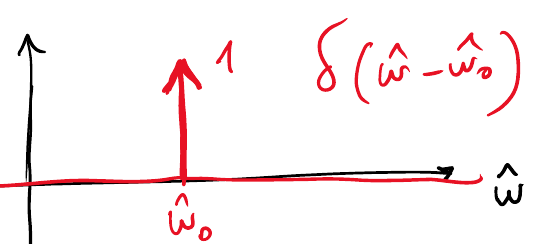
\includegraphics[scale=0.35]{immagini/lez18/deltaDirac.jpg}
\end{figure}

\subsection{Dimostrazione Empirica}
La definizione empirica di delta di Dirac e' che abbiamo una quantita' ce vale 0 tranne tra $-\hat{w}_c$ e $\hat{w}_c$ a $\pi$ dove vale $\frac{\pi}{\hat{\omega}_c}$, se consideriamo il limite di $\hat{\omega}_c \rightarrow 0$ il rettangolo si stringe alla forma limite in cui tende ad essere una $\delta(\hat{\omega})$.

\begin{figure}[ht!]
    \centering
    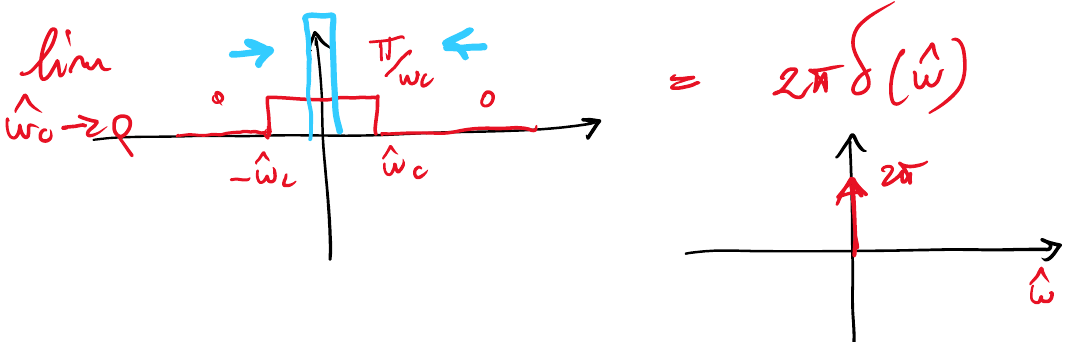
\includegraphics[scale=0.35]{immagini/lez18/diracEmpirica.jpg}
\end{figure}

\subsection{Definizione che ragiona sull'area finita}
La proprieta' del setaccio:

\[
    \int_{-\pi}^{\pi} f(\hat{\omega}) \delta(\hat{\omega} - \hat{\omega}_0) d \hat{\omega} = f(\hat{\omega})
\]

Quello che dimostra e' che la delta di Dirac e' l'integrale definito nel dominio della funzione.

\subsubsection{2}
\[
    \int_{-\pi}^{\pi} \delta(\hat{\omega} - \hat{\omega}_0) d \hat{\omega} = 1
\]

\subsubsection{3}
\[\begin{split}
    e^{j \hat{\omega}_0 n} \xleftarrow[\xrightarrow{DTFT}]{IDTFT} 2\pi \delta(\hat{\omega} - \hat{\omega}_0)
\end{split}\]

\section{Condizione sufficiente di esistenza della DTFT ("equivalente" condizioni di Dirichlet)}

Se sappiamo decomporre i segnali in componenti ortogonali capiamo come progettare un filtro. Il filtraggio in frequenza e' simile al filtraggio nel tempo, e' la stessa cosa letta in modi diversi. L'operatore per l'analisi di qualunque segnale a tempo discreto e' la DTFT, mentre l'operatore per la sintesi di qualunque segnale a tempo discreto e' la IDTFT (inverso DTFT).
Dati questi operandi troviamone le proprieta'.
Per ora non ci siamo dati condizioni di esistenza, quando possiamo applicare questi operatori?

La condizione sufficiente per l'esistenza della DTFT e' l'assoluta sommabilita' del segnale (notiamo che la condizione di Dirichlet era l'integrale nel periodo):

\begin{equation}
    \sum_{-\infty}^{+\infty} |x[n]| < + \infty
\end{equation}

Ci garantisce che qualunque segnale reale che ha un inizio ed una fine e' assolutamente sommabile e di conseguenza decomponibile. Questa condizione e' lasca nella realta', infatti nelle applicazioni pratiche si da per scontato che esista la DTFT.

Cerchiamo di darne circa una dimostrazione, vogliamo garantire che esiste (una serie esiste quando converge ad un valore finito) una DTFT, ovvero che $\sum_{-\infty}^{+\infty} x[n] e^{-j \hat{\omega}_n} = \mbox{DTFT}\{ x[n] \}$.
Quindi vuol dire che per ogni valore di $\hat{\omega}_n$ la sommatoria converge, quindi il modulo converge ma la fase puo' ruotare all'infinito, ma essendo periodica sara' sempre un multiplo di $2\pi$. Esiste significa che $|\sum_{-\infty}^{+\infty} x[n] e^{-j \hat{\omega}_n}| < +\infty$.

Se esiste la sommatoria applichiamo delle proprieta' sui coeficenti:

\[\begin{split}
    &|\sum_{-\infty}^{+\infty} x[n] e^{-j \hat{\omega}_n}| \le \sum_{-\infty}^{+\infty} |x[n] e^{-j \hat{\omega}_n}| = \sum_{-\infty}^{+\infty} |x[n]| \cancel{|e^{-j \hat{\omega}_n}|} \\
    &|\sum_{-\infty}^{+\infty} x[n] e^{-j \hat{\omega}_n}| \le \sum_{-\infty}^{+\infty} |x[n]| < + \infty
\end{split}\]

\subsection{Ulteriori riflessioni su cosa voglia dire analizzare e sintetizzare un segnale $x[n]$}

Nella prima parte del corso abbiamo parlato della sintesi tramite la serie di Fourier:

\[
    x(t) = \sum_{k = -\infty}^{+\infty} a_k e^{j 2\pi F_0 k t}
\]

mentre ora per i segnali a tempo discreto usiamo la DTFT:

\[
    x[n] = \frac{1}{2\pi} \int_{-\pi}^{+\pi} X(e^{j \hat{\omega}}) e^{j \hat{\omega}n} d\hat{\omega}
\]

In tutti e due i casi abbiamo una base su cui ricostruire il segnale, prendiamo la proiezione scalare del segnale sulla base per la base stessa.

\section{Proprieta' del ritardo temporale}
Dato un segnale e la sue DTFT lo chiameremo coppia di Fourier, se applichiamo un ritardo $n_0$ al segnale originale, otterremo :

\[\begin{split}
   x[n] &\leftrightarrow X(e^{j \hat{\omega}}) \\
   x[n - n_0] &\leftrightarrow X(e^{j \hat{\omega}}) \cdot e^{-j \hat{\omega} n_0}
\end{split}\]

Quello che succede e' che moltiplichiamo la DTFT per un termine di fase lineare che dipende da $n_0$.
Dimostriamolo:

\[\begin{split}
    DTFT\{x[n-n_0]\} &= \sum_{n = -\infty}^{+\infty} x[n-n_0] e^{-j \hat{\omega} n_0} \\
    &\mbox{Chiamiamo  } m = n - n_0 \\
    &= \sum_{m = -\infty}^{+\infty} x[m] e^{-j \hat{\omega} (m + n_0)} \\
    &= \{ \sum_{m = -\infty}^{+\infty} x[m] e^{-j \hat{\omega} m} e^{-j \hat{\omega}n_0} \}
\end{split}\]

\begin{figure}[ht!]
    \centering
    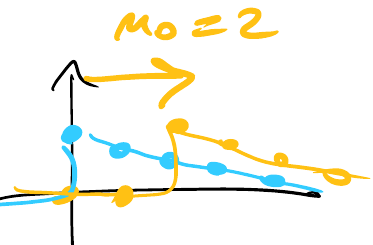
\includegraphics[scale=0.2]{immagini/lez20/ritardoTemporale.jpg}
\end{figure}


\section{Proprieta' del ritardo in frequenza}

\[\begin{split}
   x[n] &\leftrightarrow X(e^{j \hat{\omega}}) \\
   x[n] e^{j \hat{\omega}_0 n} &\leftrightarrow X(e^{j (\hat{\omega} - \hat{\omega}_0}))
\end{split}\]

\begin{figure}[ht!]
    \centering
    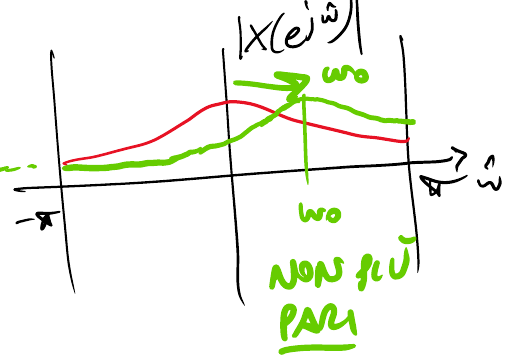
\includegraphics[scale=0.35]{immagini/lez20/ritardoFrequenza.jpg}
\end{figure}

Dimostriamolo:

\[\begin{split}
    IDTFT\{ X(e^{j(\hat{\omega}-\hat{\omega}_0)}) \} &= \frac{1}{2\pi} \int_{-\pi}^{\pi} X[e^{j(\hat{\omega}-\hat{\omega}_0)}] e^{j \hat{\omega}n} d\hat{\omega} \\
    &\mbox{Chiamiamo  } \hat{\Omega} = \hat{omega} - \hat{\omega}_0 \mbox{ e } d\hat{\omega} = d\hat{\Omega} \\
    &= frac{1}{2\pi} \int_{-\pi}^{\pi} X[e^{j(\hat{\Omega}-\hat{\omega}_0)}] e^{j (\hat{\Omega} + \hat{\omega})n} d\hat{\Omega} \\
    &= \{ frac{1}{2\pi} \int_{-\pi}^{\pi} X[e^{j(\hat{\Omega}-\hat{\omega}_0)}] e^{j\hat{\Omega}n} d\hat{\Omega} \} e^{j \hat{\omega}_0 n}
\end{split}\]

\section{Modulazione d'ampiezza}
Possiamo estendere il discorso fatto nel tempo continuo, cosa succede quando prendo il segnale e lo moltiplico per una portante, la modulazione d'ampiezza.
$x[n]$ modula l'ampiezza mentre $\cos (\hat{\omega}_0 n)$ e' la portante, noi vogliamo trovare lo spettro del segnale, e per farlo usiamo la DTFT:

\[\begin{split}
    y[n] &= x[n] \cos(\hat{\omega}_0 n) \\
    &\mbox{scomponiamo il coseno con la formula di Eulero} \\
    &= \frac{1}{2} x[n](e^{j \hat{\omega}_0 n} + e^{-j \hat{\omega}_0 n}) \\
    &= \frac{1}{2} x[n] e^{j \hat{\omega}_0 n} + \frac{1}{2} x[n] e^{-j \hat{\omega}_0 n} \\
    &\mbox{Ora calcoliamo la DTFT del segnale, per farlo usiamo la proprieta' della linearita'} \\
    DTFT\{ y[n] \} &= \frac{1}{2} \mbox{DTFT} \{ x[n] e^{j \hat{\omega}_0 n} \} + \frac{1}{2} \mbox{DTFT} \{x[n] e^{-j \hat{\omega}_0 n}\} \\
    &= \frac{1}{2} X[e^{j(\hat{\omega} - \hat{\omega}_0)}] + \frac{1}{2} X[e^{j(\hat{\omega} + \hat{\omega}_0)}]
\end{split}\]

\begin{figure}[ht!]
    \centering
    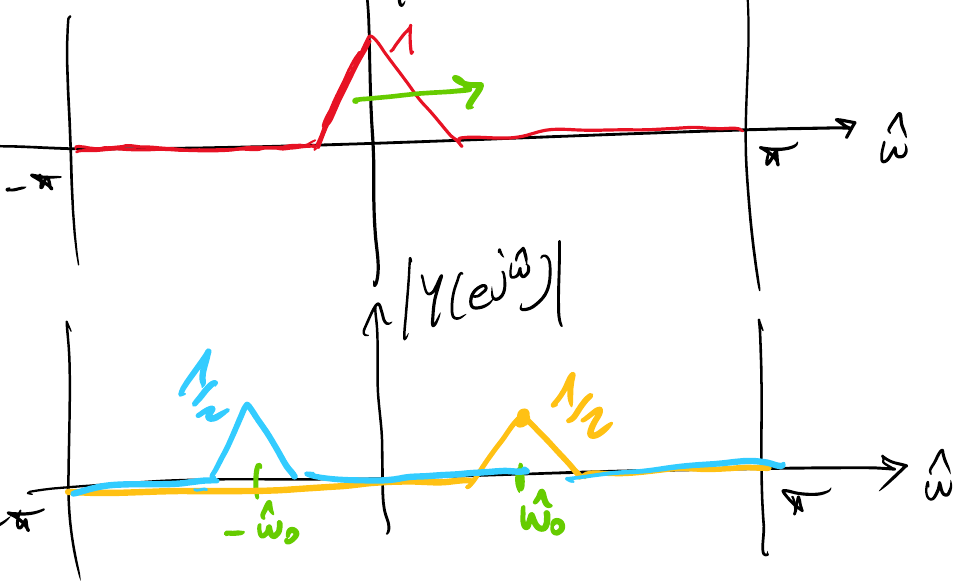
\includegraphics[scale=0.35]{immagini/lez20/modulazioneAmpiezza.jpg}
\end{figure}

\section{Spettro di un coseno}
Ricordiamo:

\[\begin{split}
    x[n] &= 1 \leftrightarrow X(e^{j \hat{\omega}}) = \delta(\hat{\omega})2\pi \\
    y[n] &= x[n] \cos(\hat{\omega}_0 n) = \cos(\hat{\omega}_0 n)
\end{split}\]

Ora vogliamo calcolare la DTFT del coseno, ed intuitivamente abbiamo l'idea che il risultato di una decomposizione di un coseno deve essere un coseno, verifichiamolo:

\[\begin{split}
    \mbox{DTFT}\{ \cos(\hat{\omega}_0 n) \} &= \mbox{DTFT} \{ \frac{1}{2} e^{j \hat{\omega}_0 n} + \frac{1}{2} e^{-j \hat{\omega}_0 n} \} \\
    &= \frac{1}{2} \mbox{DTFT} \{ e^{j \hat{\omega}_0 n} \} + \frac{1}{2} \mbox{DTFT} \{ e^{-j \hat{\omega}_0 n} \} \\
    &= \frac{2\pi}{2} \delta(\hat{\omega} - \hat{\omega}_0) + \frac{2\pi}{2} \delta(\hat{\omega} + \hat{\omega}_0)
\end{split}\]

\begin{figure}[ht!]
    \centering
    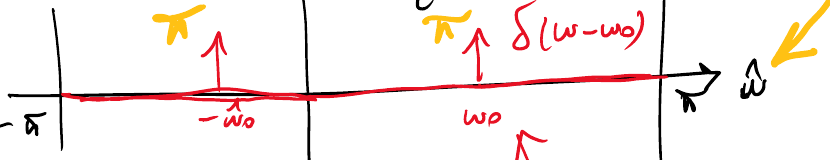
\includegraphics[scale=0.35]{immagini/lez20/spettroCoseno.jpg}
\end{figure}

Quindi lo spettro di un coseno ha solo una linea spettrale alla frequenze del coseno (come ci aspettiamo dalla formula di Eulero).

\section{Proprieta' DTFT della convoluzione}
E' una proprieta' molto importante, perche' ci permette di fare tante cose. Si utilizzano dei metodi spettrali, in cui un problema si cerca di risolverlo nel dominio spettrale perche' e' piu' facile.

Quello che ci dice questa proprieta' e' che la convoluzione di due segnali nel dominio nel tempo viene trasformata in un prodotto in quello delle frequenze (dopo aver trasformato i segnali tramite la DTFT):

\[\begin{split}
    &\mbox{TEMPO:  } z[n] = x[n] * y[n] = \sum_{k = -\infty}^{+\infty} x[n-k] y[k] \\
    &\mbox{Applicando la DTFT ai segnali:} \\
    &\mbox{FREQUENZE:  } Z(e^{j\hat{\omega}}) = X(e^j\hat{\omega}) \cdot Y(e^{j\hat{\omega}})
\end{split}\]

Dimostriamolo:

\[\begin{split}
    \mbox{DTFT} \{ z[n] \} &= \sum_{n=-\infty}^{+ \infty} z[n]e^{-j\hat{\omega}n} = \sum_{n=-\infty}^{+\infty} \sum_{k=-\infty}^{+\infty} x[n-k] y[k] e^{-j \hat{\omega}n} \\
    &= \sum_{k=-\infty}^{+\infty} y[k] \sum_{n=-\infty}^{+\infty} x[n-k] e^{-j \hat{\omega}n} \\
    &\mbox{Ricordando la proprieta' 5: DTFT } \{ x[n-k] \} = X(e^{j\hat{\omega}}) e^{-j\hat{\omega}k} \\
    &= \{ \sum_{k=-\infty}^{+\infty} y[k] e^{-j \hat{\omega}k} \} X(e^{j \hat{\omega}}) = Y(e^{j\hat{\omega}}) X(e^{j\hat{\omega}})
\end{split}\]

\section{Esercizio 1}
Facciamo ora degli esercizi per utilizzare le proprieta' della DTFT.
Come primo esercizio consideriamo come segnale una composizione lineare di delta:

\[
    x[n] = 2\delta[n+3] - \delta[n] - \delta[n-1] + 2\delta[n+1] + 5\delta[n-7]
\]

Ora utilizziamo la proprieta' di linearita' della DTFT ricordando inoltre che la DTFT di una delta e' 1 ed applichiamo anche la proprieta' del ritardo:

\[
    X(e^{j\hat{\omega}}) = 2 \cdot 1 e^{-j \hat{\omega}(-3)} -1 \cdot 1 e^{-j \hat{\omega}(0)} -1 \cdot 1 e^{-j \hat{\omega}(1)} + 2 \cdot 1 e^{-j \hat{\omega}(-1)} + 5 \cdot 1 e^{-j \hat{\omega}(7)}
\]

\section{Esericio 2}
Ora consideriamo come segnale il segnale rettangolo, che e' un segnale che vale 1 tra 0 ed $L-1$, e vale 0 altrimenti.

\begin{figure}[ht!]
    \centering
    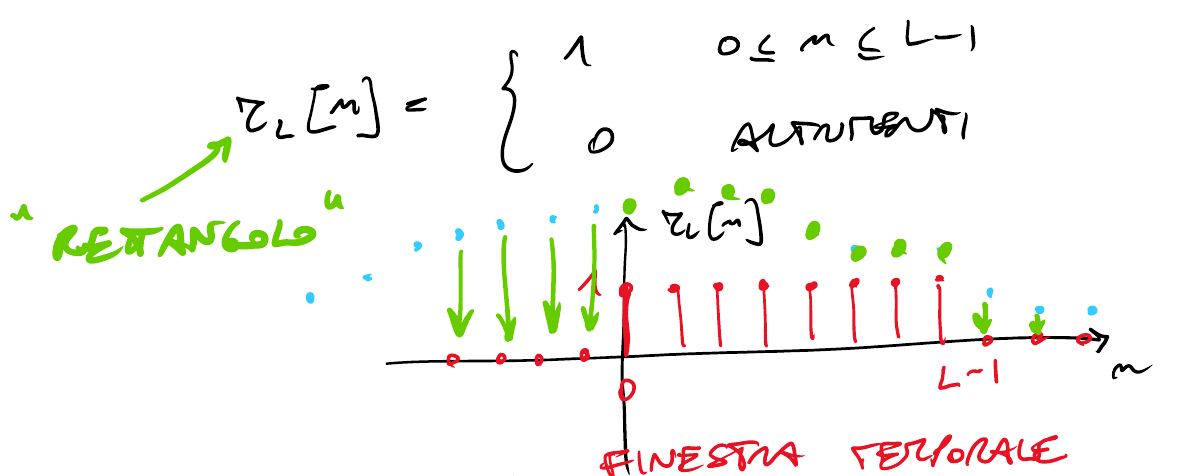
\includegraphics[scale=0.35]{immagini/lez21/es2Rettangolo.jpg}
\end{figure}

Moltiplicare per la finestra rettangolo per qualsiasi segnale significa focalizzarci su $L-1$ campioni. Vediamo ora la DTFT del segnale:

\[\begin{split}
    DTFT\{r_L [n]\} &= \sum_{n = -\infty}^{+\infty} r_L [n] e^{-j \hat{\omega}n} = \sum_{n=0}^{L-1}(e^{-j\hat{\omega}})^n \\
    &= \frac{1-q^L}{1-q} = \frac{1-e^{-j\hat{\omega}L}}{1-e^{-j\hat{\omega}}} \\
    &= e^{-j \hat{\omega} \frac{(L-1)}{2}} \frac{\sin \hat{\omega} \frac{L}{2}}{\sin\frac{\hat{\omega}}{2}} = R_L(e^{j\hat{\omega}})
\end{split}\]

Abbiamo ottenuto la forma di Dirichlet

\begin{figure}[ht!]
    \centering
    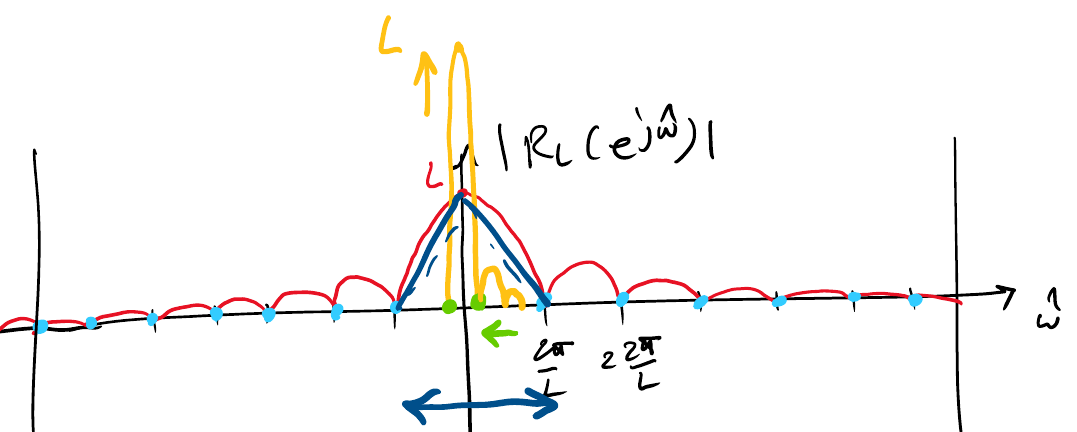
\includegraphics[scale=0.35]{immagini/lez21/es2ModuloRettangolo.jpg}
\end{figure}

Notiamo anche che se portiamo al limite l'area del primo lobo otteniamo una delta di dirac.

\section{Esempio 3}
Utilizziamo ora un segnale rettangolo per filtrare un segnale coseno :

\[\begin{split}
    x[n] &= \cos(\hat{\omega}_0 n) \leftrightarrow \pi \delta(\hat{\omega} - \hat{\omega}_0) + \pi \delta(\hat{\omega} + \hat{\omega}_0) \\
    \Tilde{x[n]} &= \cos(\hat{\omega}_0 n) r_L[n] \leftrightarrow \frac{1}{2} R_L (e^{j(\hat{\omega} - \hat{\omega}_0)}) + \frac{1}{2} R_L (e^{j(\hat{\omega} + \hat{\omega}_0)})
\end{split}\]

\begin{figure}[ht!]
    \centering
    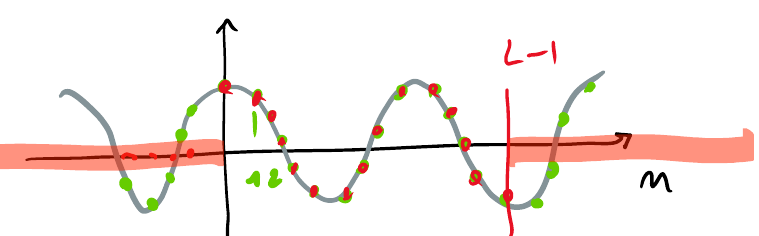
\includegraphics[scale=0.35]{immagini/lez21/filtraggioRettangolo.jpg}
\end{figure}

Ora calcoliamo la DTFT di questo segnale:

\[\begin{split}
    \mbox{DTFT}\{\Tilde{x[n]}\} &= \frac{1}{2} \mbox{DTFT} \{ e^{j \hat{\omega}_0 n} r_L[n] \} + \frac{1}{2} \mbox{DTFT} \{ e^{-j \hat{\omega}_0 n} r_L[n] \} \\
    &= \frac{1}{2} R_L(e^{j (\hat{\omega} - \hat{\omega}_0)}) + \frac{1}{2} R_L(e^{j (\hat{\omega} + \hat{\omega}_0)})
\end{split}\]

Tracciandone il grafico del modulo  e notiamo che quando ricostruiamo un segnale da uno troncato, otteniamo due lobi centrati dovo sono le componenti del coseno, nel caso in cui faccio tendere L all'infinito trovo esattamente la delta di Dirac.

\begin{figure}[ht!]
    \centering
    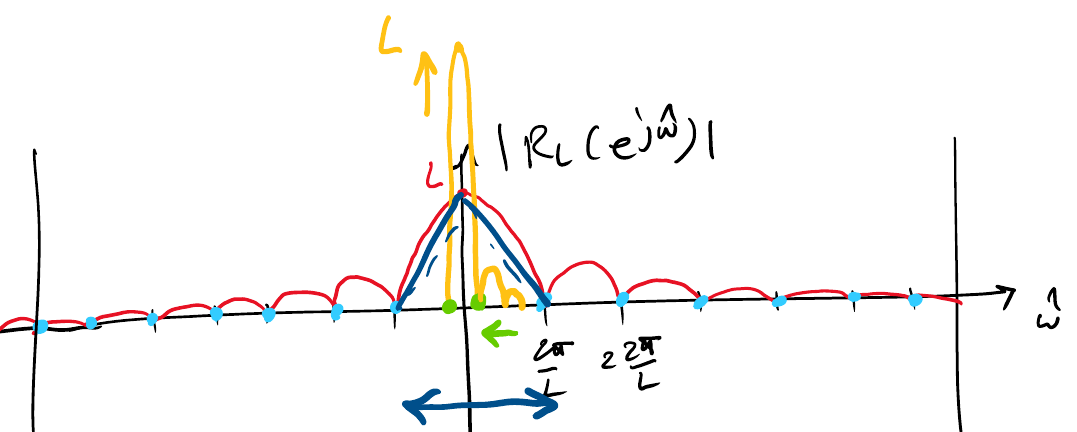
\includegraphics[scale=0.35]{immagini/lez21/es2ModuloRettangolo.jpg}
\end{figure}

\section{Teorema di Parseval (legge di conservazione) per segnali tempo discreti}
Prima di dare questo teorema diamo una definizione di \underline{energia di un segnale tempo discreto}: 

\begin{equation}
    E = \sum_{n= - \infty}^{+\infty} |x[n]|^2
\end{equation}

Diciamo che il teorema di Parseval passa dal dominio del tempo al dominio delle frequenze:

\begin{equation}
    E = \sum_{n= -\infty}^{+\infty} |x[n]|^2 = \frac{1}{2\pi} \int_{-\pi}^{\pi} |X(e^{j\hat{\omega}})|^2 d\hat{\omega}
\end{equation}

\begin{figure}[ht!]
    \centering
    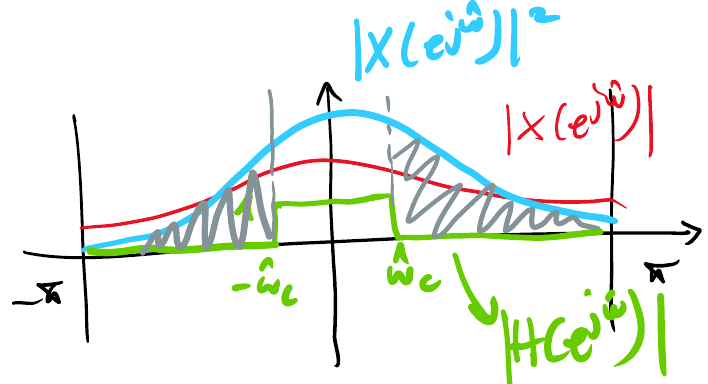
\includegraphics[scale=0.35]{immagini/lez21/teoremaParseval.jpg}
\end{figure}

Quello che succede in pratica e' che ci dice quant'e' l'energia associata a ciascuna delle frequenze del segnale.

Dimostriamolo per passi:

\subsection{Passo 1 dimostrazione}
Ribaltiamo la DTFT nel tempo e nelle frequenze:

\[\begin{split}
    \mbox{DTFT}\{x[-n]\} &= X()e^{-j \hat{\omega}} \\
    \mbox{DTFT}\{x^*[n]\} &= X^*(e^{-j\hat{\omega}})
\end{split}\]

\subsection{Passo 2 dimostrazione}
\[\begin{split}
    &\mbox{DTFT}\{x^*[n] * x[-n]\} = \\
    &\mbox{DTFT}\{x^*[n]\} \cdot \mbox{DTFT}\{x[-n]\} = \\
    &X^*(e^{-j\hat{\omega}}) \cdot X(e^{-j\hat{\omega}}) = 
    |X(e^{-j\hat{\omega}})|^2
\end{split}\]

Per un segnale reale e' la densita' spettrale di energia.

\subsection{Passo 2 dimostrazione}
\[\begin{split}
    x^*[n] * x[-n] &= \sum_{k = -\infty}^{+\infty} x*[n] x[-(n-k)] \\
    &= \sum_{k = -\infty}^{+\infty} x*[n] x[k-n] \\
    x^*[n] * y[n] &= \sum_{k = -\infty}^{+\infty} x[k] y[n-k]
\end{split}\]


\subsection{Passo 4 dimostrazione}

\[\begin{split}
    &\mbox{DTFT} \{x^*[n] * x[-n]\} = |X(e^{-j\hat{\omega}})|^2 \\
    &x^*[n] * x[-n] = \mbox{IDTFT} \{|X(e^{-j\hat{\omega}})|^2\} \\
\end{split}\]

Concludendo:

\begin{equation}
    \sum_{k = -\infty}^{+\infty} x^*[n] * x[k-n] = \frac{1}{2\pi} \int_{-\pi}^{\pi} |X(e^{-j\hat{\omega}})|^2 e^{j\hat{\omega}n} d\hat{\omega}
\end{equation}

Per i segnali reali togliamo i coniugati complessi ed $n=0$:

\[
    \sum_{k = -\infty}^{+\infty} |x[n]|^2 = \frac{1}{2\pi} \int_{-\pi}^{\pi} |X(e^{j\hat{\omega}})|^2 d\hat{\omega}
\]

\section{Matched Filter}

\begin{figure}[ht!]
    \centering
    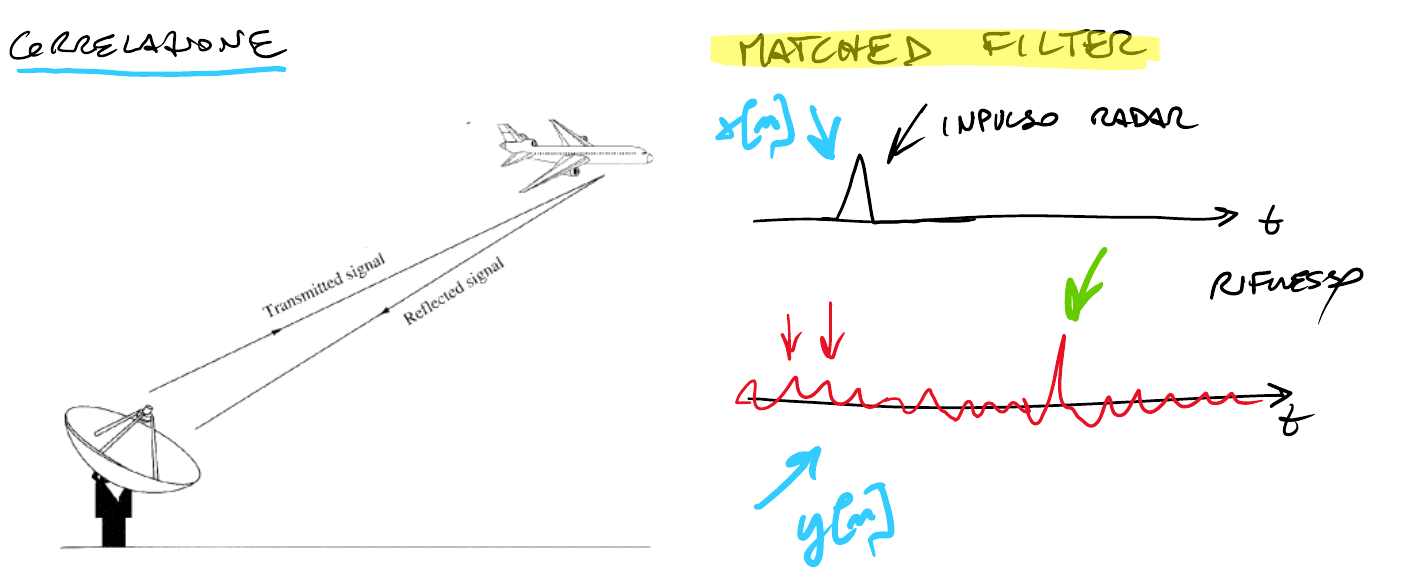
\includegraphics[scale=0.35]{immagini/lez22/matchedFilter.jpg}
\end{figure}

Il matched filter serve per localizzare occorrenze di un segnale in un altro (in presenza di rumore). Calcolando la (cross-)correlazione di un template o maschera con il segnale. La correlazione e' massima quando sono identici.

\section{Precisazione cambio di variabile}
Quando ricostruiamo un segnale tramite la IDTFT possiamo farlo nel mondo del tempo utilizzando l'integrale tra $-\pi$ e $\pi$, oppure possiamo farlo nel mondo delle frequenze cambiando variabile:

\[\begin{split}
    x[n] &= \frac{1}{2\pi} \int_{-\pi}^{\pi} X(e^{j\hat{\omega}}) e^{j\hat{\omega}n} d\hat{\omega} \\
    \hat{f} &= \frac{\hat{\omega}}{2\pi} \Rightarrow d\hat{f} = \frac{d\hat{\omega}}{2\pi} \\
    &= \frac{1}{\cancel{2\pi}} \int_{\frac{-\pi}{2\pi} = -\frac{1}{2}}^{\frac{\pi}{2\pi} = \frac{1}{2}} X(e^{j2\pi\hat{f}}) e^{j2\pi\hat{f}n} \cancel{2\pi} d\hat{f}
\end{split}\]

\section{Risposta in frequenza e DTFT}
Torniamo a parlare della risposta in frequenza, sappiamo che l'uscita di un sistema LTI e' la convoluzione tra il segnale in ingresso e la sua risposta all'impulso.
Dato che sappiamo che la DTFT se esiste e' unica, allora :

\[\begin{split}
    \mbox{DTFT}\{y[n]\} &= \mbox{DTFT}\{x[n] * h[n]\} \\
    Y(e^{j\hat{\omega}} &= X(e^{j\hat{\omega}}) \cdot \mbox{DTFT}\{h[n]\} \\
    \mbox{DTFT}\{h[n]\} &= \sum_{n=-\infty}^{+\infty} h[n] e^{-j \hat{\omega} n_0} = H(e^{j\hat{\omega}})
\end{split}\]

Abbiamo quindi trovato un terzo modo per vedere la risposta in frequenze che e' la DTFT del sistema e possiamo trovarla dal rapporto tra la DTFT dell'uscita del sistema e la DTFT dell'ingresso del sistema:

\[\begin{split}
    Y(e^{j\hat{\omega}} &= X(e^{j\hat{\omega}}) \cdot H(e^{j\hat{\omega}}) \\
    H(e^{j\hat{\omega}}) &= \frac{Y(e^{j\hat{\omega}}}{X(e^{j\hat{\omega}})}
\end{split}\]

\section{Filtraggio (LTI) nel tempo vs frequenze}

\begin{figure}[ht!]
    \centering
    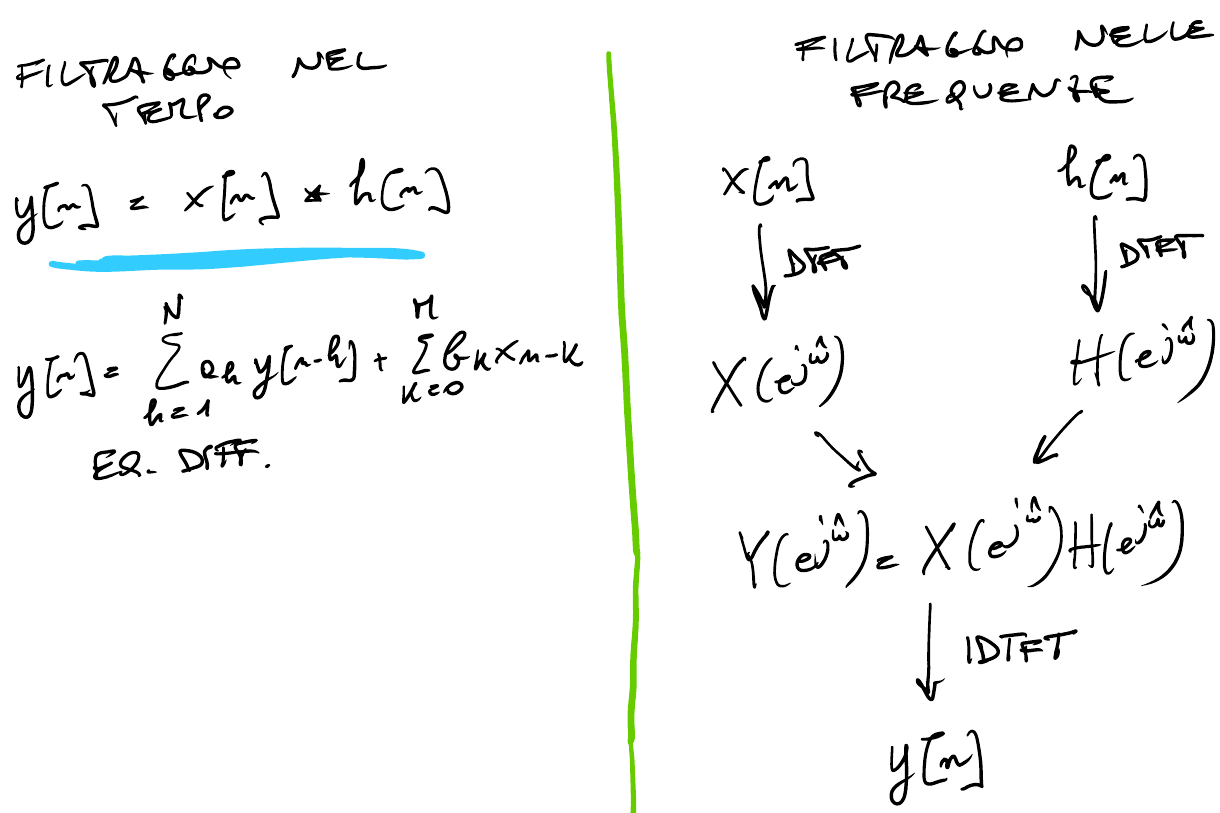
\includegraphics[scale=0.35]{immagini/lez22/filtraggioTempoFrequenze.jpg}
\end{figure}

Da questa chiarificazione notiamo che a volte puo' essere piu' semplice portarsi nel dominio delle frequenze per fare il filtraggio, in modo tale che la convoluzione si trasformi in una moltiplicazione.

Possiamo ancora ragionare sul filtraggio LTI, posso calcolare la DTFT di un segnale ed ottenere il modulo della DTFT, poi dato che voglio filtrare moltiplico quel modulo per il modulo della risposta all'impulso del filtro che mi interessa (nel nostro caso un filtro passa basso), faccio una moltiplicazione punto punto ed ottengo il modulo dell'uscita del sistema.

\begin{figure}[ht!]
    \centering
    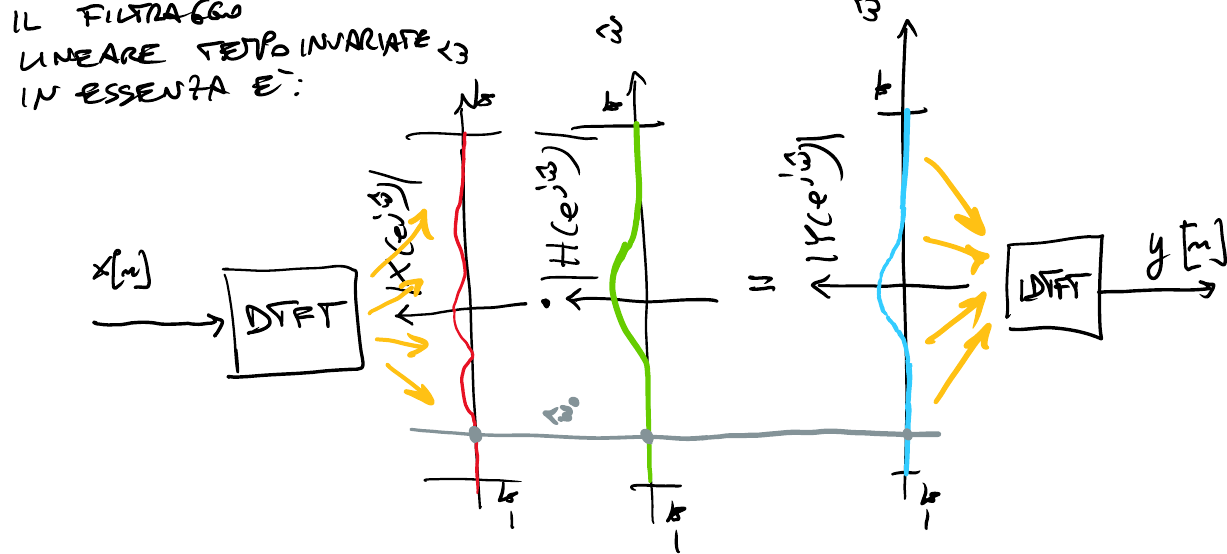
\includegraphics[scale=0.35]{immagini/lez22/filtraggioLTI.jpg}
\end{figure}

\section{Un primo esempio di sistema LIT IIR}
Fino ad ora abbiamo considerato sistemi FIR. Ora sappiamo anche manipolare sistemi LTI con risposta all'impulso infinita.
Vediamo un primo esempio di sistema LTI IIR:

\[\begin{split}
    y[n] &= \frac{1}{2} y[n-1] + x[n] \\
    x[n] &= \delta[n]
\end{split}\]

Notiamo subito che c'e' la parte autoregressiva quindi e' probabile che il sistema sia IIT, vogliamo trovare l'output del sistema.

Calcoliamo l'output del sistema nei punti in cui e' diverso da 0:

\[\begin{split}
    y[-2] &= h[-2] = 0 \\
    y[-1] &= h[-1] = 0 \\
    y[0] &= h[0] = 1 = (\frac{1}{2})^0\\
    y[1] &= \frac{1}{2} \cdot 1 + 0 = \frac{1}{2} = (\frac{1}{2})^1\\
    y[2] &= \frac{1}{2} \cdot \frac{1}{2} + 0 = \frac{1}{4} = (\frac{1}{2})^2\\
    y[3] &= \frac{1}{2} \cdot \frac{1}{4} + 0 = \frac{1}{8} = (\frac{1}{2})^3\\
\end{split}\]

Da questi punti notiamo che il segnale in uscita ha un andamento del tipo:

\[
    y[n] = h[n] = (\frac{1}{2})^n u[n]
\]

\begin{figure}[ht!]
    \centering
    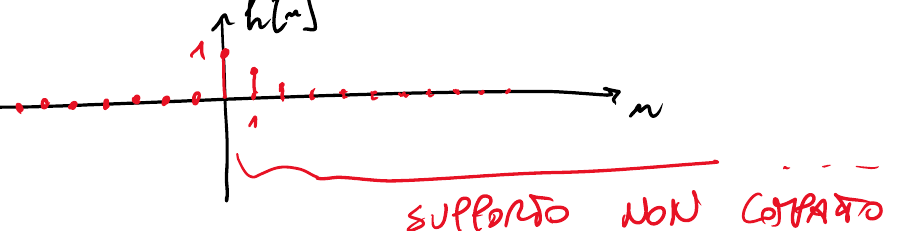
\includegraphics[scale=0.35]{immagini/lez22/es1.jpg}
\end{figure}

Ora per calcolare la risposta in frequenza utilizziamo le coppie di DTFT che abbiamo usato in precedenza per vedere se possiamo ricondurci a qualcuna di esse:

\[
    H(e^{j\hat{\omega}}) = \sum_{n=-\infty}^{+\infty} h[n] e^{-j\hat{\omega}n} = DTFT\{h[n\} = \frac{1}{1 - \frac{1}{2} e^{-j\hat{\omega}}}
\]

Abbiamo risolto questo esercizio in 3 passaggi, siamo partiti dall'equazione alle differenze, abbiamo trovato la risposta all'impulso ed infine abbiamo calcolato la risposta in frequenza, proviamo a farlo in un passaggio solo passando direttamente dall'equazione alle differenze alla risposta in frequenza.

\begin{figure}[ht!]
    \centering
    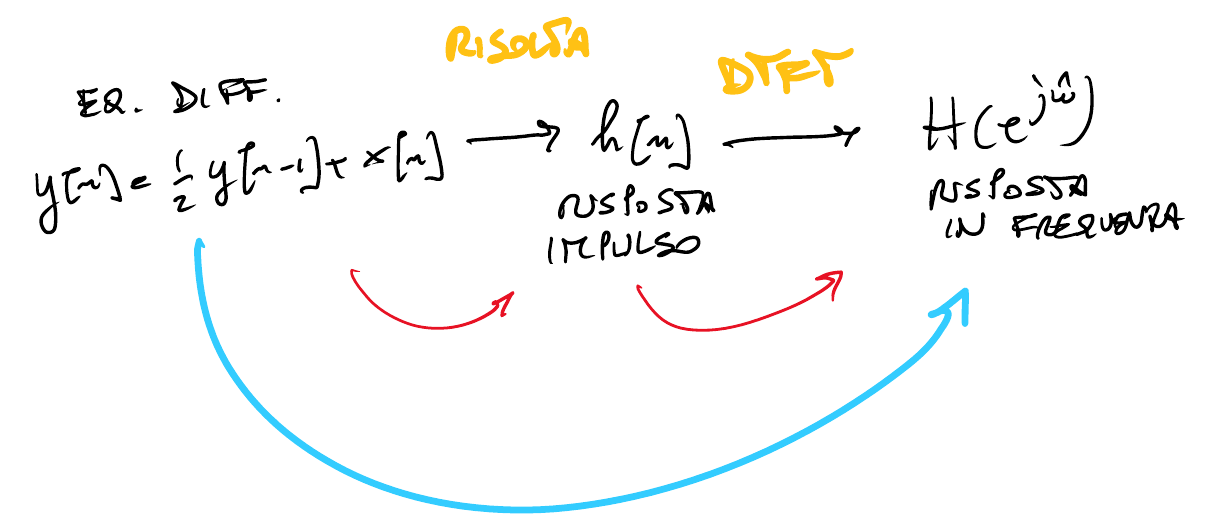
\includegraphics[scale=0.35]{immagini/lez22/es13passaggi.jpg}
\end{figure}

\[\begin{split}
    y[n] &= \frac{1}{2} y[n-1] + x[n] \rightarrow \mbox{ usiamo la proprieta' dell'unicita' della DTFT} \\
    \mbox{DTFT}\{y[n]\} &= \mbox{DTFT}\{\frac{1}{2} y[n-1] + x[n]\} \rightarrow \mbox{ usiamo la proprieta' di linearita'} \\ 
    Y(e^{j\hat{\omega}}) &= \frac{1}{2} \mbox{DTFT}\{y[n-1]\} + \mbox{DTFT}\{x[n]\} \rightarrow \mbox{ ora applichiamo la proprieta' del ritardo} \\
    Y(e^{j\hat{\omega}}) &= \frac{1}{2} Y(e^{j\hat{\omega}}) e^{-j \hat{\omega}1} + X(e^{j\hat{\omega}}) \\
    Y(e^{j\hat{\omega}}) (1 - \frac{1}{2} e^{-j\hat{\omega}}) &= X(e^{j\hat{\omega}}) \\
    \frac{Y(e^{j\hat{\omega}})}{X(e^{j\hat{\omega}})} &= \frac{1}{1-\frac{1}{2}e^{-j\hat{\omega}}} 
\end{split}\]

Lo stesso ragionamento lo possiamo fare per qualunque equazione alle differenze:

\[\begin{split}
    y[n] &= \sum_{h = -N_1, h \neq 0}^{N_2} ah y[n-h] + \sum_{h = -M_1, h \neq 0}^{M_2} bk x[n-k] \\
    &\mbox{Proprieta' di unicita'} \\
    \mbox{DTFT} \{y[n]\} &= \mbox{DTFT} \{\sum_{h = -N_1, h \neq 0}^{N_2} ah y[n-h] + \sum_{h = -M_1, h \neq 0}^{M_2} bk x[n-k]\} \\
    &\mbox{Proprita' di linearita'}\\
    Y(e^{j\hat{\omega}}) &= \sum_{h = -N_1, h \neq 0}^{N_2} ah \mbox{DTFT} \{y[n-h]\} + \sum_{h = -M_1, h \neq 0}^{M_2} bk \mbox{DTFT} \{x[n-k]\} \\
    &\mbox{Proptieta' del ritardo} \\
    Y(e^{j\hat{\omega}}) \{1- \sum_{h = -N_1, h \neq 0}^{N_2} ah e^{-j\hat{\omega}h}\} &= X(e^{j\hat{\omega}}) \{1- \sum_{h = -M_1, h \neq 0}^{M_2} bk e^{-j \hat{\omega}k}\} \\
    \frac{Y(e^{j\hat{\omega}})}{X(e^{j\hat{\omega}})} &= \frac{\sum_{h = -M_1, h \neq 0}^{M_2} bk e^{-j \hat{\omega}k}}{\sum_{h = -N_1, h \neq 0}^{N_2} ah e^{-j\hat{\omega}h}}
\end{split}\]

\section{Esercizio}
Dato un equazione alle differenze di un sistema LTI:

\[
    y[n] = \frac{9}{10} y[n-1] + \frac{1}{20} x[n] + \frac{1}{20} x[n-1]
\]

calcolare la risposta in frequenza e poi la risposta all'impulso.
Cominciamo calcolando la risposta in frequenza usando le proprieta' di unicita', linearita' e del ritardo come abbiamo fatto fino ad adesso:

\[\begin{split}
    &Y(e^{j\hat{\omega}}) = \frac{9}{20} Y(e^{j\hat{\omega}})e^{-j\hat{\omega} 1} + \frac{1}{20} X(e^{j\hat{\omega}}) + \frac{1}{20} X(e^{j\hat{\omega}})e^{-j\hat{\omega}1} \\
    &Y(e^{j\hat{\omega}}) \{1-\frac{9}{10}e^{-j\hat{\omega}}\} = X(e^{j\hat{\omega}})\{\frac{1}{20} + \frac{1}{20}e^{-j\hat{\omega}}\} \\
    &\frac{Y(e^{j\hat{\omega}})}{X(e^{j\hat{\omega}})} = \frac{\frac{1}{20}(1+e^{-j\hat{\omega}})}{1-\frac{9}{10}e^{-j\hat{\omega}}} = H(e^{j\hat{\omega}})
\end{split}\]

Per trovare la risposta all'impulso dobbiamo calcolare $h[n] = IDTFT\{H(e^{j\hat{\omega}}\}$, per farlo andiamo a vedere le proprieta' e le coppie di DTFT per vedere se possiamo riscrivere H in modo da ricondurci a delle coppie note:

\[\begin{split}
    H(e^{j\hat{\omega}}) &= \frac{1}{20} \cdot \frac{1}{1-\frac{9}{10}e^{-j\hat{\omega}}} + \frac{1}{20}e^{e^{-j\hat{\omega}}} \cdot \frac{1}{1-\frac{9}{10} e^{-j\hat{\omega}}} \\
    h[n] &= \frac{1}{20} \cdot (\frac{9}{10})^n u[n] + \frac{1}{20} \cdot (\frac{9}{10})^{n-1} u[n-1]
\end{split}\]

\section{DFT}
\begin{figure}[ht!]
    \centering
    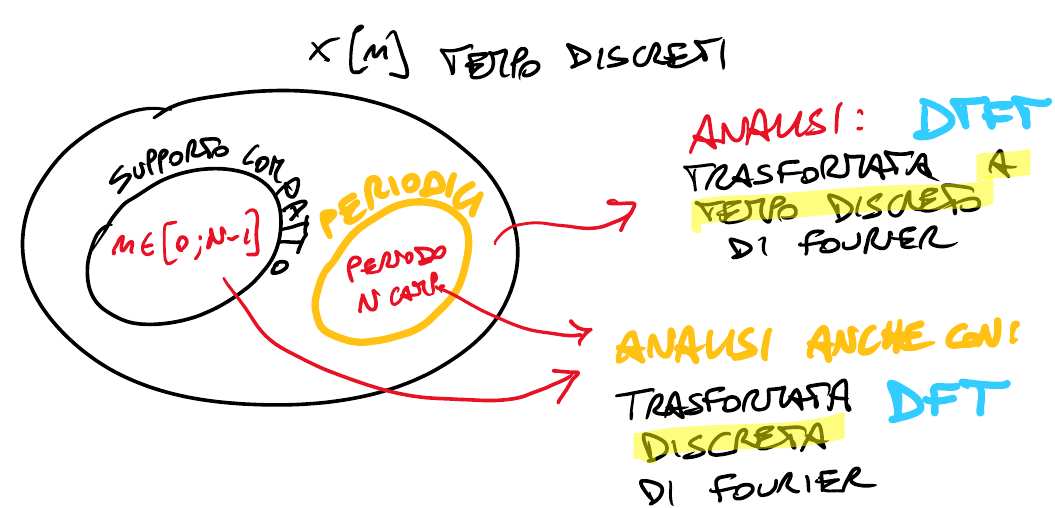
\includegraphics[scale=0.35]{immagini/lez23/segnaliDFT.jpg}
\end{figure}

In realta' i sottoinsiemi di segnali che ci interessano, ovvero i segnali a supporto compatto e/o periodici, possono essere analizzati tramite un operatore piu' comodo della DTFT, la \underline{trasformata discreta di Fourier DFT}.

Sappiamo che la DTFT di un segnale e':

\[
    \mbox{DTFT}\{x[n]\} = X(e^{j\hat{\omega}}) = \sum_{n = \cancel{-\infty} 0 }^{\cancel{+\infty} N-1} x[n] e^{-j\hat{\omega}n}
\]

Dato che stiamo prendendo in considerazione solo segnali a supporto compatto possiamo ridurre la sommatoria ad $n \in [0, N-1]$, inoltre possiamo discretizzare la frequenza, ovvero prendiamo un numero limitato di campioni perche' se nella DTFT $\hat{\omega} \in \mathbf{R} (-\pi; +\pi]$, nella DFT consideriamo $\hat{\omega}_k = \frac{2\pi}{N}\cdot k \rightarrow k\in[0; N-1]$. Quindi concludendo la DFT di un segnale e':

\begin{equation}
    \mbox{DFT}\{x[n]\} X_{[k]} = \sum_{n=0}^{N-1} x[n] e^{-j\frac{2\pi}{N} \cdot kn}
\end{equation}

\begin{figure}[ht!]
    \centering
    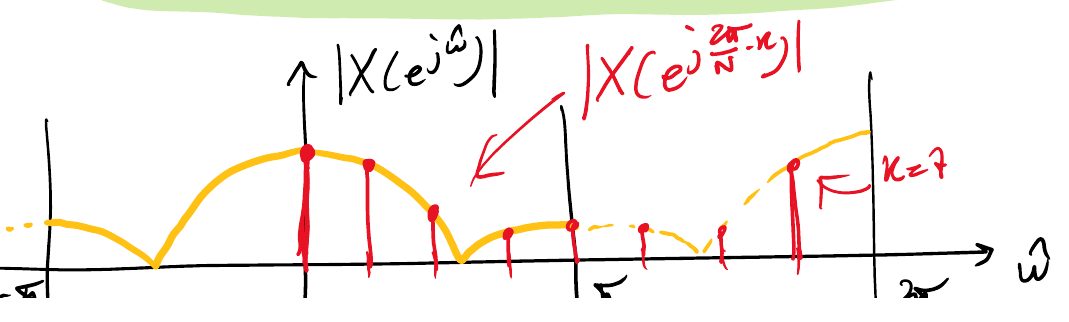
\includegraphics[scale=0.35]{immagini/lez23/moduloDFT.jpg}
\end{figure}

Esiste anche una formula di sintesi la IDFT:

\[
\mbox{IDFT}\{x_{[k]}\} = \frac{1}{N} \sum_{n=0}^{N-1} x[n] e^{j\frac{2\pi}{N} \cdot kn}
\]

\medskip
\medskip
\medskip
\medskip
\medskip
\medskip
\medskip
\medskip
\medskip
\medskip
\medskip
\medskip
\medskip
\medskip
\medskip
\medskip
\medskip
\medskip
\medskip
\medskip
\medskip
\medskip
\medskip
\medskip
\medskip
\medskip
\medskip
\medskip
\medskip
\medskip
\medskip
\medskip
\medskip
\medskip
\medskip
\medskip
\medskip
\medskip
\medskip
\medskip
\medskip
\medskip
\medskip
\medskip
\medskip
\medskip
\medskip
\medskip
\medskip
\medskip
\medskip
\medskip
\medskip
\medskip
\medskip
\medskip
\medskip
\medskip
\medskip
\medskip
\medskip
\medskip
\medskip
\medskip
\medskip
\medskip
\medskip
\medskip
\medskip
\medskip
\medskip
\medskip
\medskip
\medskip
\medskip
\medskip
\medskip
\medskip
\medskip
\medskip
\medskip
\medskip
\medskip
\medskip
\medskip
\medskip
\medskip
\medskip
\medskip
\medskip
\medskip
\medskip
\medskip

\subsection{Esercizio}

\begin{figure}[ht!]
    \centering
    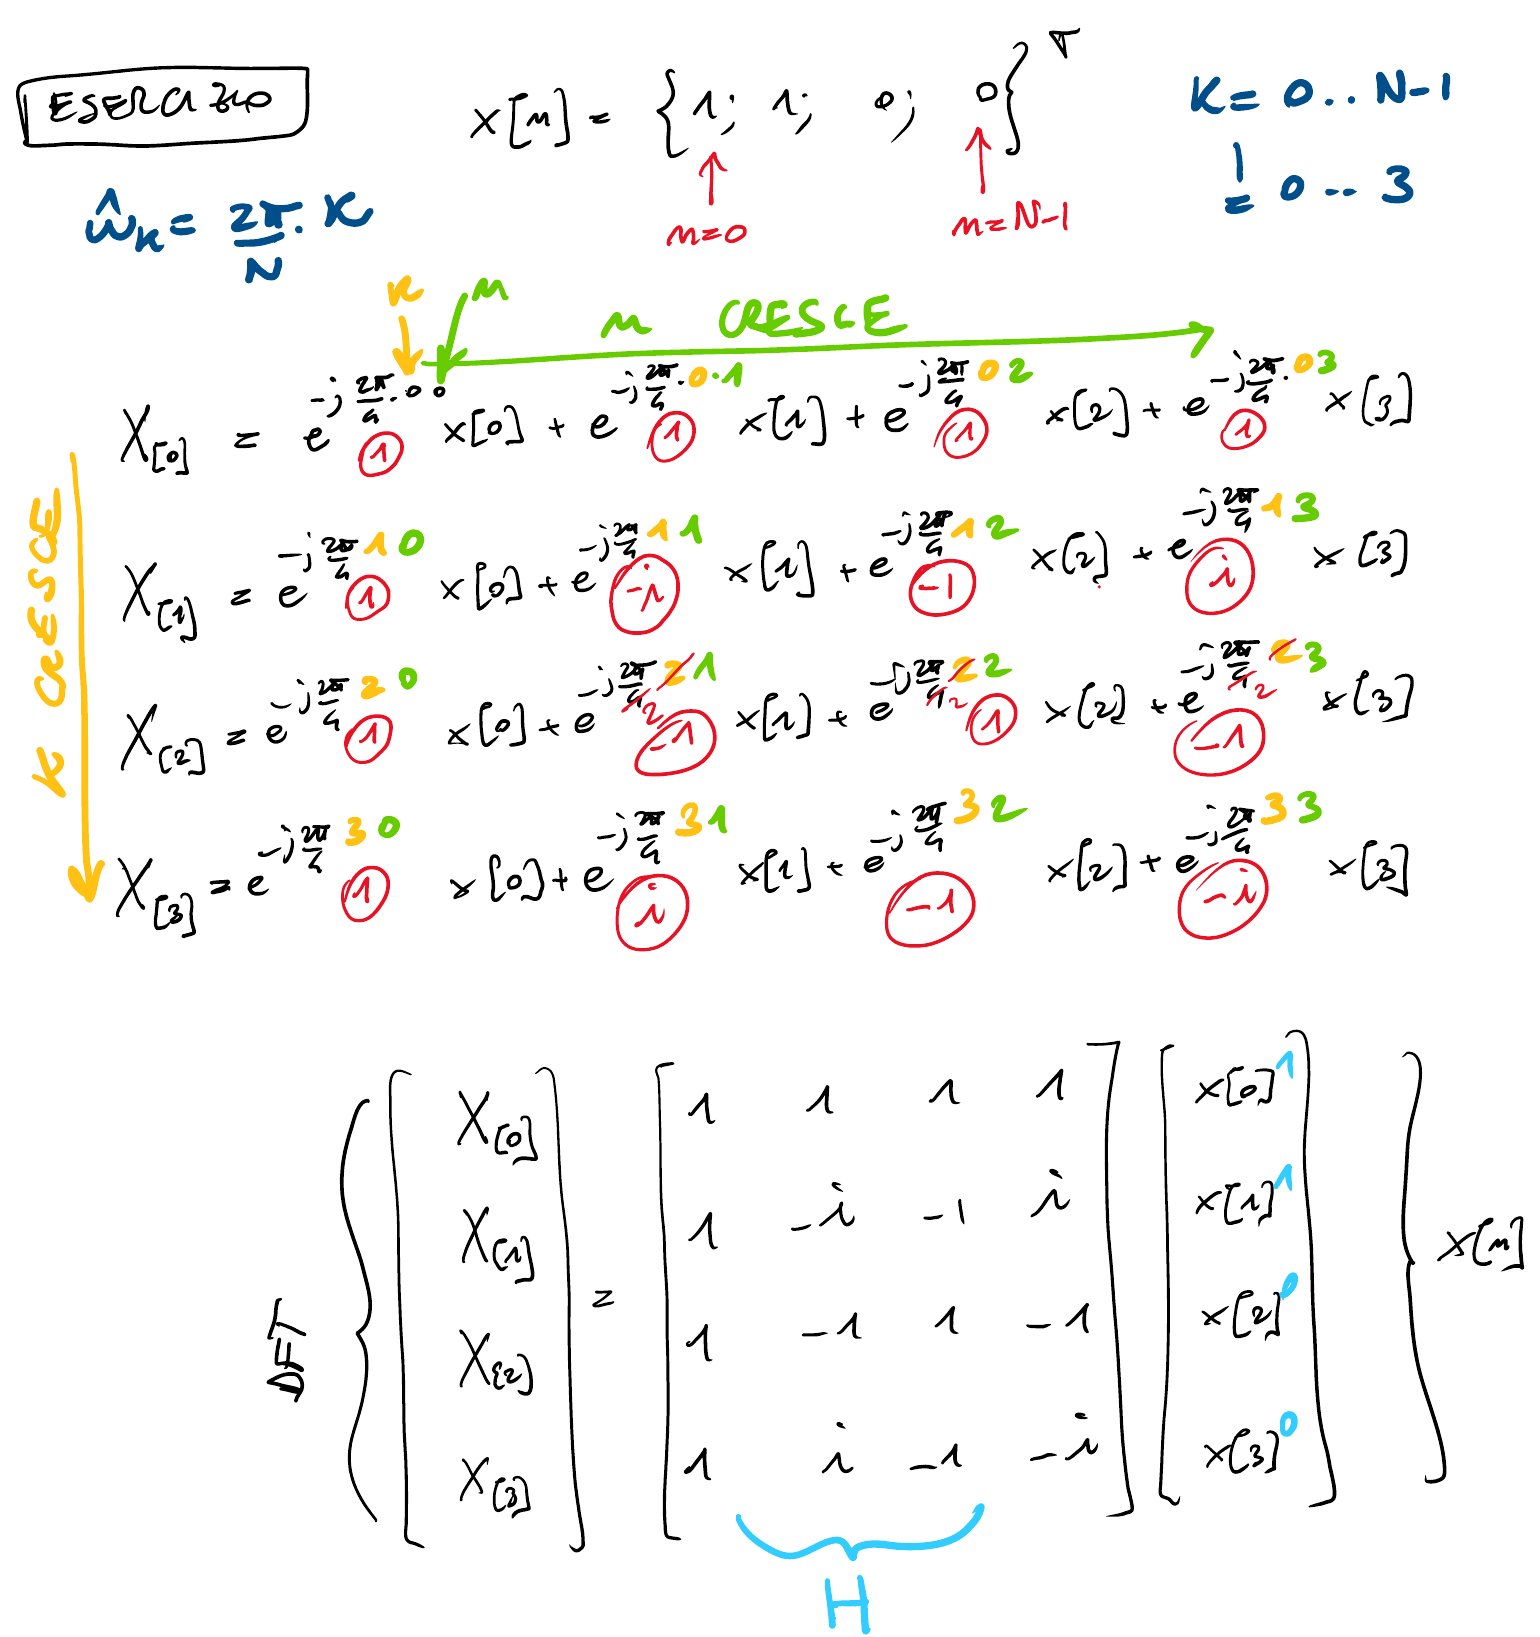
\includegraphics[scale=0.35]{immagini/lez23/esercizio.jpg}
\end{figure}


Abbiamo fatto un esercizio per vedere come funziona la DFT per un vettore di 4 elementi, quindi sappiamo che in questo caso $k=3$ ed N pure, quello che abbiamo fatto e' stato calcolare elemento per elemento la DFT sostituendo opportunamente k ed N nella formula. Successivamente abbiamo visto quanto valgono gli esponenziali complessi (i numeri cerchiati in rosso), ed abbiamo notato che quindi quello che succede e' come se moltiplicassimo il segnale per una matrice H, ed i punti che otteniamo sono:

\[\begin{split}
    X_[0] = 2 \rightarrow \hat{\omega}_{k=0} = \frac{2\pi}{4} \cdot 0 = 0 \\
    X_[1] = 1 - i \rightarrow \hat{\omega}_{k=1} = \frac{2\pi}{4} \cdot 1 = \frac{\pi}{2} \\
    X_[2] = 0 \rightarrow \hat{\omega}_{k=2} = \frac{2\pi}{4} \cdot 2 = \pi \\
    X_[3] = 1 + i \rightarrow \hat{\omega}_{k=3} = \frac{2\pi}{4} \cdot 3 = \frac{3}{2}\pi \\
\end{split}\]

\begin{figure}[ht!]
    \centering
    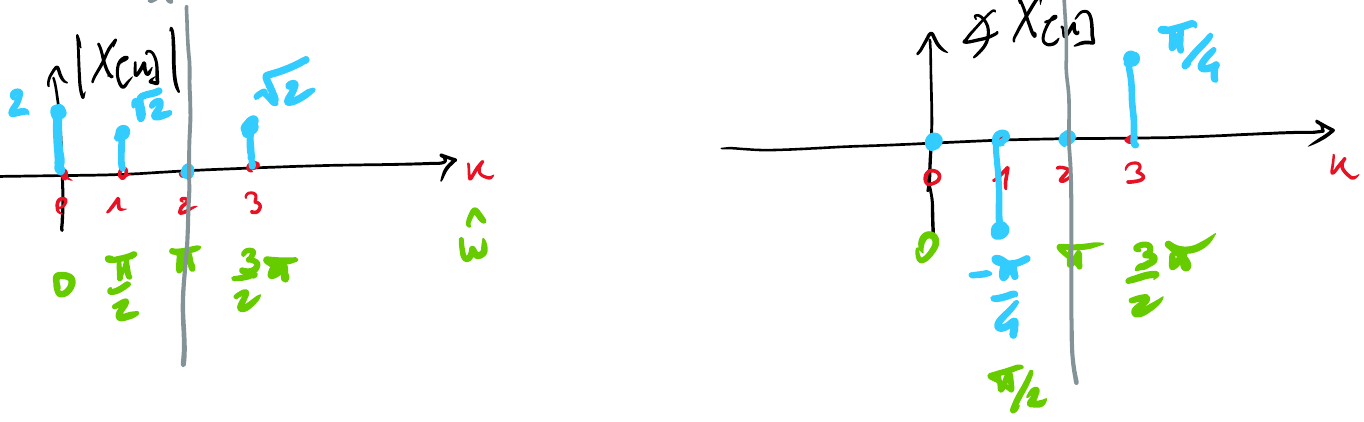
\includegraphics[scale=0.35]{immagini/lez23/moduloFaseEsercizio.jpg}
\end{figure}

Tracciando il grafico del modulo e della fase notiamo che non sono simmetrici, questo perche' abbiamo considerato la simmetria fuori dall'alias principale.

Quindi concludendo possiamo dire che la DFT di un segnale (vettore) e' il segnale stesso moltiplicato per la matrice H:

\[
    \mbox{DFT: } X_[k] = H x[n]
\]

di conseguenza possiamo riscrivere la IDFT come il segnale moltiplicato per la matrice coniugata (coniugato di elemento per elemento della matrice) e trasposta (ruotata sulla diagonale):

\[
    \mbox{IDFT: } x[n] = H^{-1} X_[k] = \frac{1}{N}(H^*)^T \cdot X_[k]
\]

Per avere in riscontro di quello fatto adesso in questo esercizio, calcoliamo la DTFT del vettore per vedere se troviamo gli stessi punti:

\[\begin{split}
    \mbox{DTFT}\{[1100]\} &= 1 + e^{-j\hat{\omega}} = 2e^{-j\frac{\hat{\omega}}{2}} (\frac{e^{j\frac{\hat{\omega}}{2}} + e^{j\frac{\hat{\omega}}{2}}}{2}) \\
    &= 2e^{-j\frac{\hat{\omega}}{2}} \cos \frac{\hat{\omega}}{2}
\end{split}\]

Tracciamo il grafico del modulo e della fase:

\begin{figure}[ht!]
    \centering
    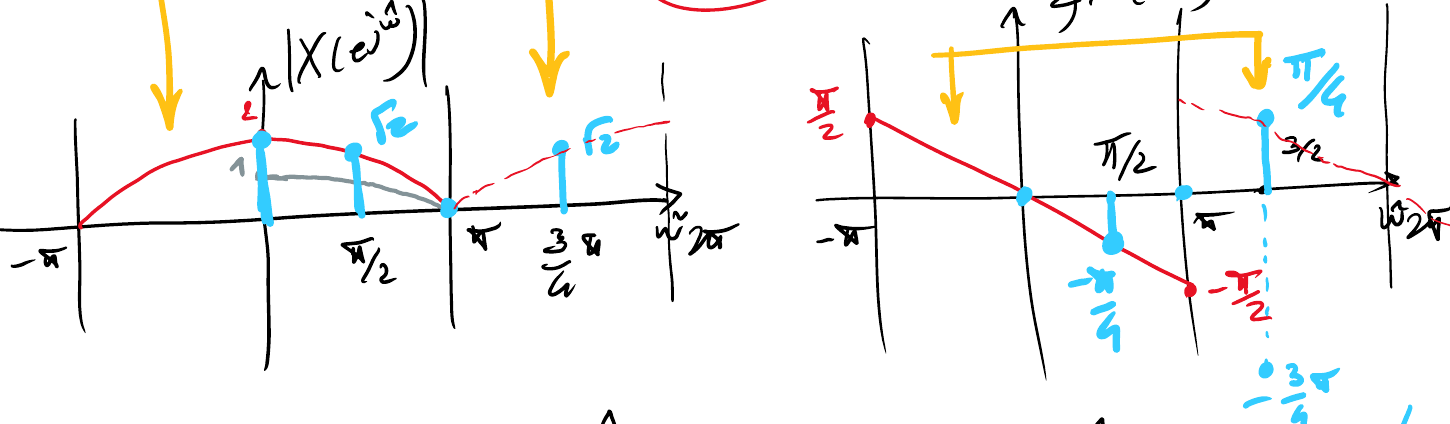
\includegraphics[scale=0.35]{immagini/lez23/moduloFaseEs1.jpg}
\end{figure}

Ora calcoliamo la DTFT per ogni punto del vettore per vedere se ottengo gli stessi punti che abbiamo trovato prima:

\[\begin{split}
    \hat{\omega} &= 0 \rightarrow X(e^{j\hat{\omega}}) = 2 \\
    \hat{\omega} &= \frac{\pi}{2} \rightarrow X(e^{j\hat{\omega}}) = 2cos\frac{\pi}{4} e^{-j\frac{\pi}{4}} \\
    \hat{\omega} &= \pi \rightarrow X(e^{j\hat{\omega}}) = 2cos\frac{\pi}{2} e^{-j\frac{\pi}{2}} \\
    \hat{\omega} &= \frac{3}{2}\pi \rightarrow X(e^{j\hat{\omega}}) = 2cos\frac{3}{4} \pi e^{-j\frac{3}{4}\pi} \\
\end{split}\]

\section{Proprieta' della DFT}
Vediamo le varie proprieta' della DFT come abbiamo fatto in precedenza per la DTFT

\subsection{Proprieta' 1: DFT periodica di N punti}
A differenze della DTFT che era periodica di $2\pi$ la DFT e' periodica di N punti:

\[\begin{split}
    &k \rightarrow \frac{2\pi}{N} \cdot k = \hat{\omega} \\
    X_[k] &= \sum_{n=0}^{N-1} x[n] e^{-j \frac{2\pi}{N}\cdot kn} \\
    X_[k+n] &= \sum_{n=0}^{N-1} x[n] e^{-j \frac{2\pi}{N}(k+N)n} \\
    &= \sum_{n=0}^{N-1} x[n]e^{-j \frac{2\pi}{N} \cdot kn} \cdot \cancel{e^{-j \frac{2\pi}{\cancel{N}}\cdot n \cancel{N}}} \\
    X_[k+n] &= X_[k]
\end{split}\]

\subsection{Propritea' 2: DFT e' simmetrica coniugata se $x[n] \in \mathbf{R}$ }

La DTFT e' simmetrica coniugata se il segnale e' reale, il che vuol dire che $X(e^{-j\hat{\omega}}) = X^*(e^{j\hat{\omega}})$, quindi avevamo una simmetria dei campioni che si "ribaltavano" sull'asse y. Mentre con la DFT abbiamo una simmetria ma su $\pi$.

Quindi quello che succede per il modulo e' che ho un campione iniziale $k=0$ che e' centrato sull'asse y, poi ho una serie di campioni che vengono copiati uguali e ribaltati sul campione centrale $k = \frac{N}{2} + 1$. Mentre con la fase ho sempre un campione iniziale ed uno centrale, ed i campioni tra quello iniziale e centrale vengono ribaltati e copiati cambiati di segno.
Notiamo che il campione centrale esiste solamente se N e' pari, inoltre facciamo attenzione al fatto che il campione iniziale $k=0$ ed il campione centrale in $\pi$ DEVONO essere numeri Reali.

\begin{figure}[ht!]
    \centering
    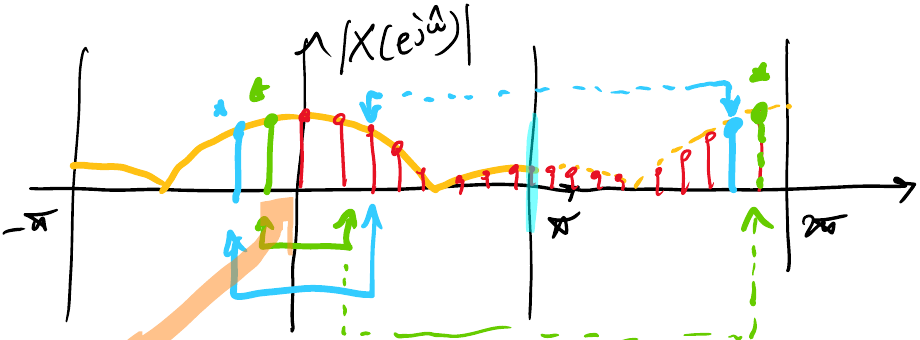
\includegraphics[scale=0.35]{immagini/lez24/DFTsimmetricaConiugata.jpg}
\end{figure}

\begin{figure}[ht!]
    \centering
    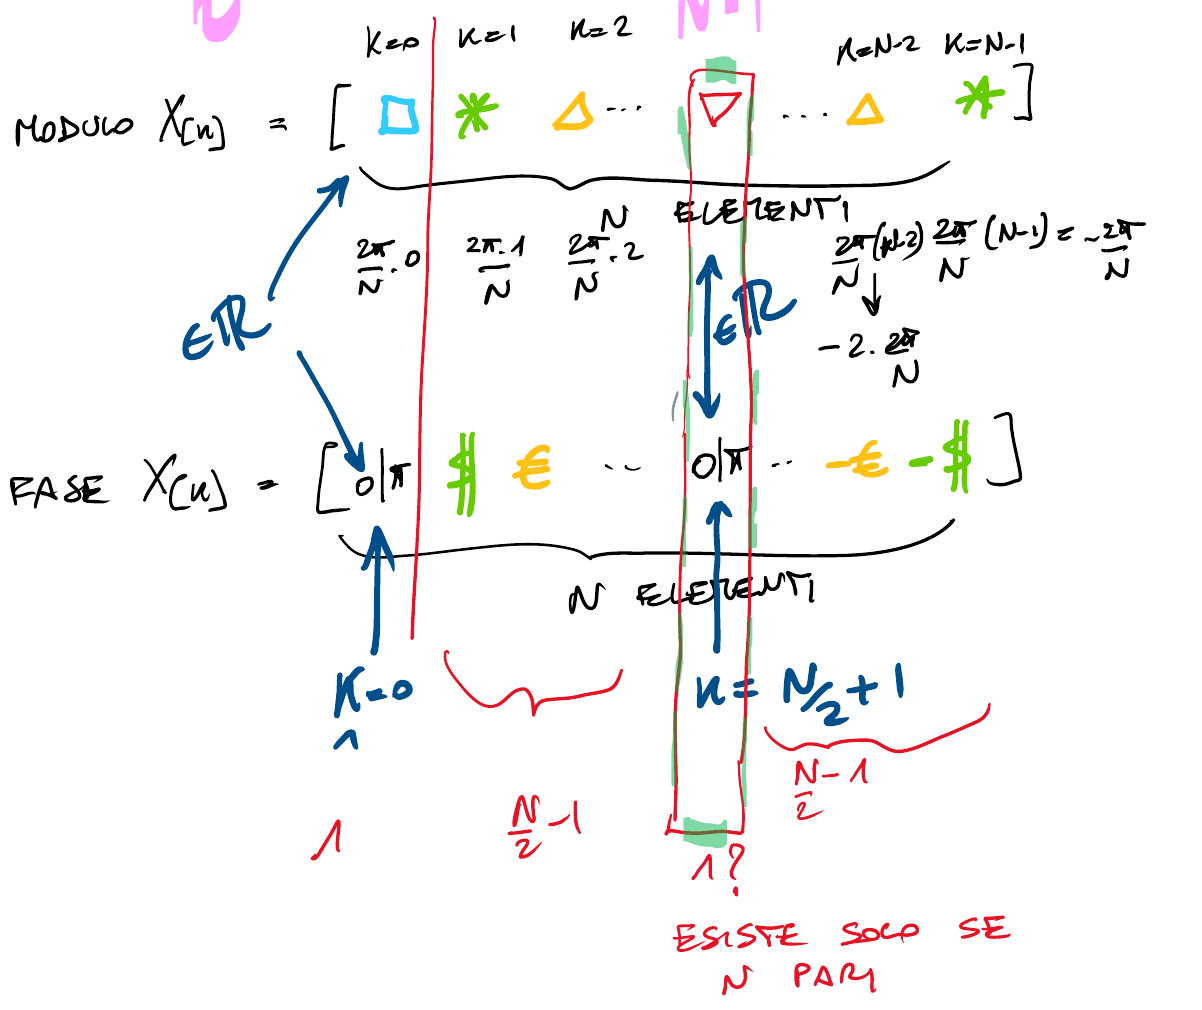
\includegraphics[scale=0.30]{immagini/lez24/DTFesempio.jpg}
\end{figure}


\subsubsection{Esercizio}
Facciamo un esercizio per vedere data una DFT se il segnale era reale.
Abbiamo un vettore di 8 elementi, quindi N e' pari di conseguenza avremo il campione centrale a $\pi$ che nel nostro caso e' il posizione 4 del vettore ed e' uguale a $1+i$.
Ora passo passo verifichiamo che le condizioni date prima sono verificate, il campione in posizione $k=0$ e quello centrale in posizione $\pi$ sono due numeri reali, quindi va bene. Poi verifichiamo che le varie coppie siano coniugati complessi, e vediamo subito che la prima coppia (ovvero l'elemento in posizione 1 e l'ultimo, quello in posizione 7) non sono coniugati complessi. Quindi possiamo subito concludere che il segnale non era reale.

\begin{figure}[ht!]
    \centering
    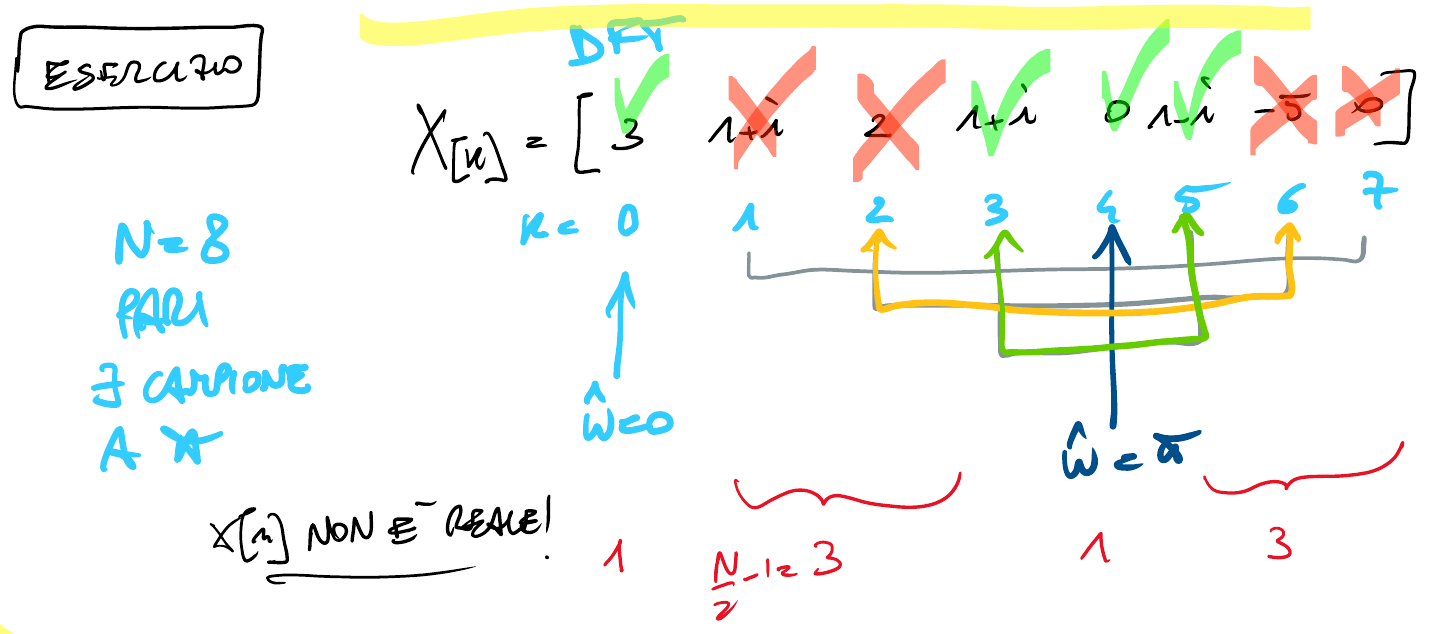
\includegraphics[scale=0.35]{immagini/lez24/esercizioDFT.jpg}
\end{figure}

\subsection{Proprieta' 4: DFT e' unica}
La DFT, che esiste sempre, e' unica solo per segnali periodici. Il segnale $x[n]$ a supporto compatto $[0; N-1]$ ha la stessa DFT di un segnale periodico $X_p[n]$ di periodo N avente periodo base uguale a $x[n]$ per $n \in [0; N-1]$.

\begin{figure}[ht!]
    \centering
    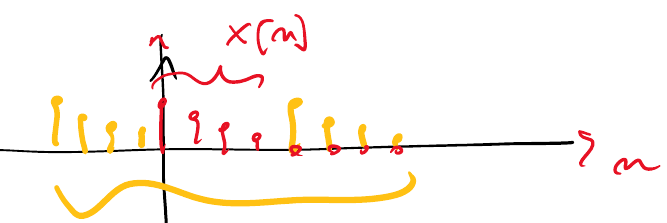
\includegraphics[scale=0.35]{immagini/lez24/prop4.jpg}
\end{figure}

\subsection{Proprieta' 5: ritardo temporale}
Ricordiamo la proprieta' del ritardo temporale per la DTFT:

\[
    \mbox{DTFT} x[n-n_0] \leftrightarrow X(e^{j\hat{\omega}})e^{-j\hat{\omega}n_0}
\]

Vediamo cosa succede se ritardiamo la DFT, partiamo ricordando com'e' fatta la DFT di un segnale:

\[
    x[n] = \frac{1}{N} \sum_{k=0}^{N-1} X_[k]e^{-j \frac{2\pi}{N} \cdot kn}
\]

\begin{figure}[ht!]
    \centering
    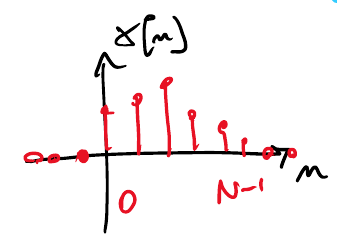
\includegraphics[scale=0.35]{immagini/lez24/x[n]Prop5.jpg}
\end{figure}

ora ritardiamo il segnale sostituendo $n+N$ ad n:

\[\begin{split}
    x[n+N] &= \frac{1}{N} \sum_{k=0}^{N-1} X_[k]e^{-j \frac{2\pi}{N} (n+N) \cdot k}\\
    &= \sum_{n=0}^{N-1} x[n]e^{-j \frac{2\pi}{N} \cdot kn} \cdot \cancel{e^{-j \frac{2\pi}{\cancel{N}}\cdot n \cancel{N}}} \\
    X_[n+N] &= X_[n]
\end{split}\]

Quindi attenzione perche' la ricostruzione rende periodico il segnale. La $x[n]$ corrisponde sia alla DFT di un segnale a supporto compatto che a quella di uno periodico.

\begin{figure}[ht!]
    \centering
    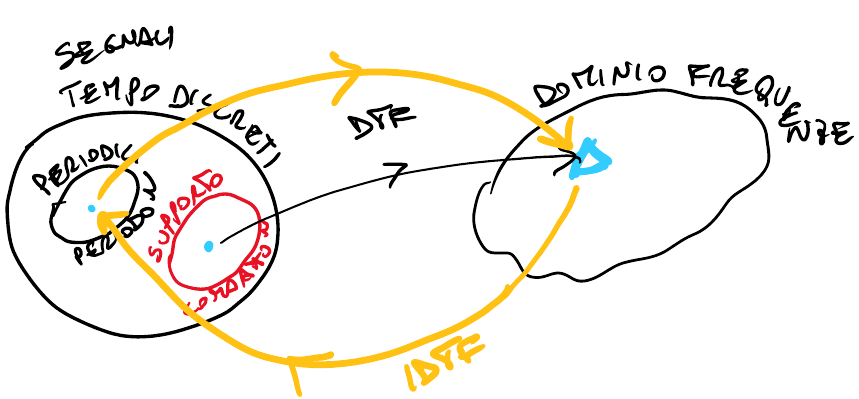
\includegraphics[scale=0.35]{immagini/lez24/DFTperiodica.jpg}
\end{figure}

Questo pero' e' un problema, in quanto se trasliamo un segnale che e' stato ricostruito e reso periodico, nell'alias principale entrano dei campioni che generano rumore e non vorremmo:

\begin{figure}[ht!]
    \centering
    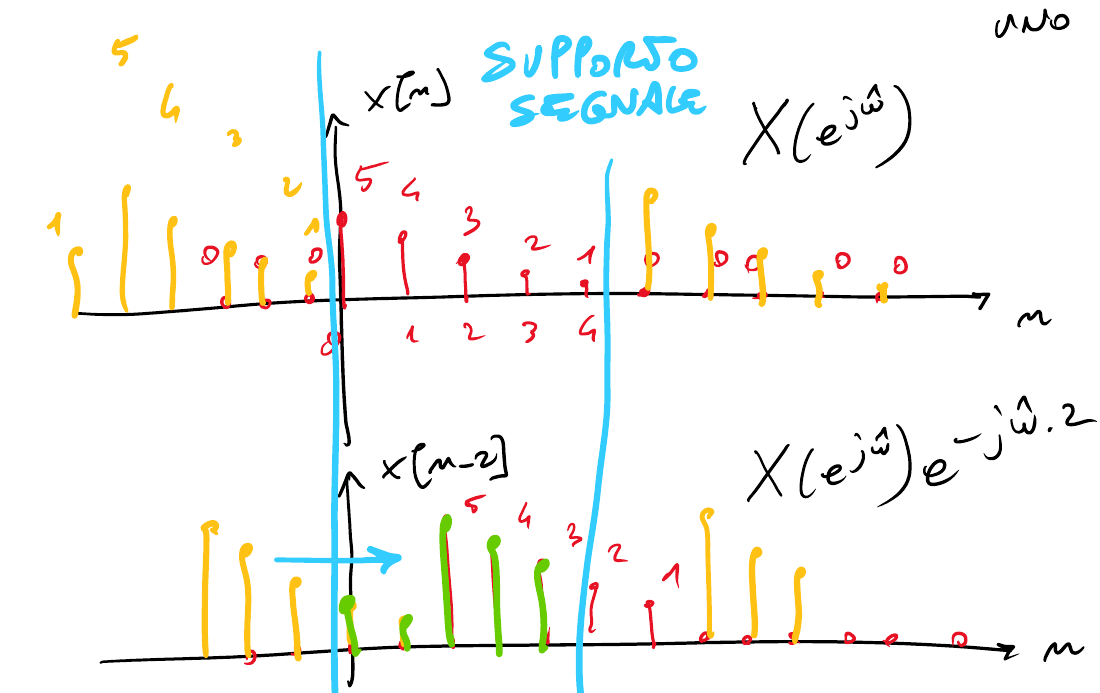
\includegraphics[scale=0.35]{immagini/lez24/DFTaliasSecondari.jpg}
\end{figure}

\begin{figure}[ht!]
    \centering
    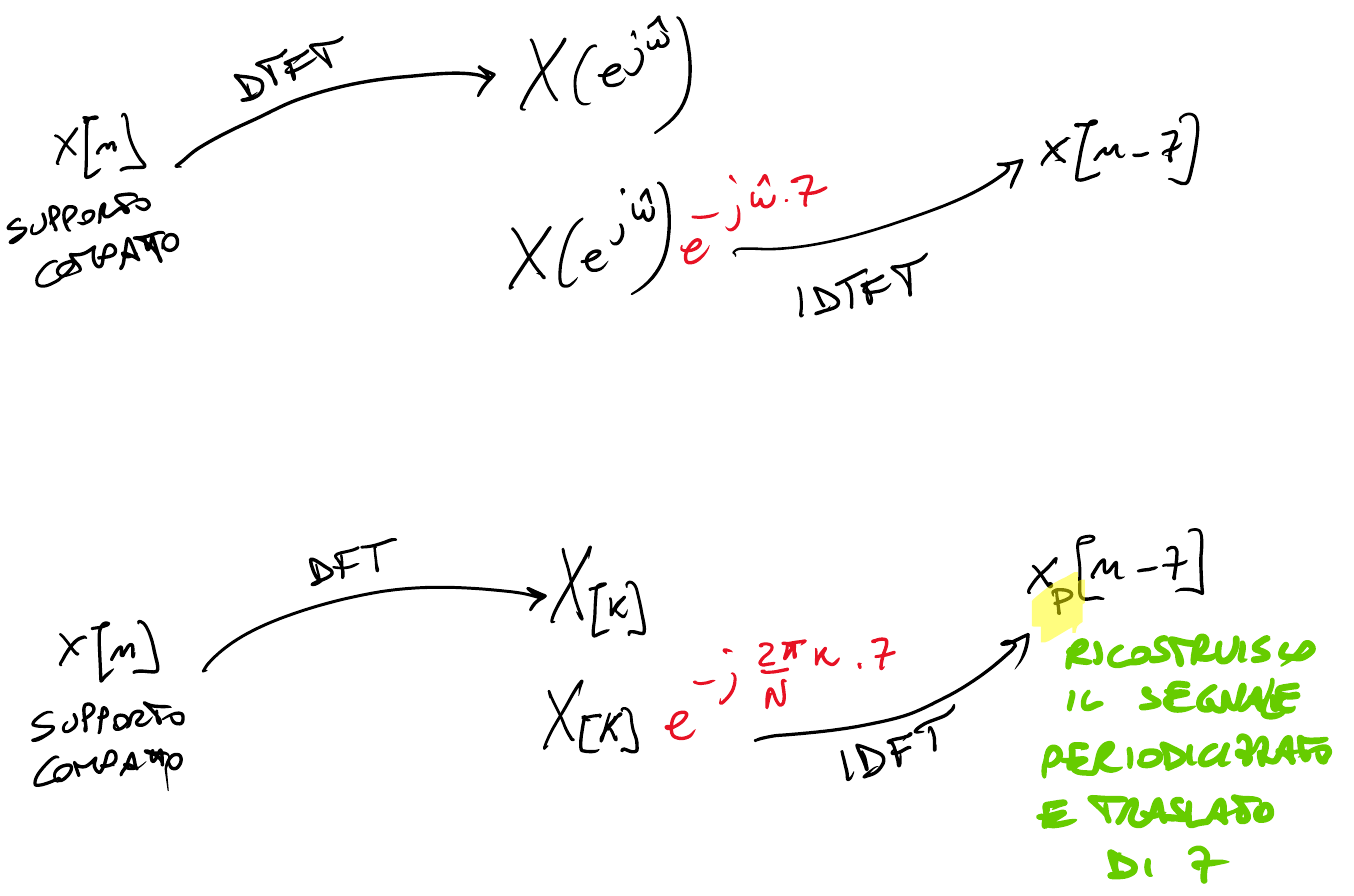
\includegraphics[scale=0.35]{immagini/lez24/DFTIDTFT.jpg}
\end{figure}


\subsection{Proprieta' 6: convoluzione}
La convoluzione la usiamo spesso per filtrare un segnale, ma vale anche tra due segnali.
Sappiamo che per trvare l'uscita di un sistema LTI dobbiamo fare la convoluzione tra l'input del sistema e la risposta all'impulso. 
Usano la DTFT non abbiamo problemi :

\[
y[n] = IDTFT \{DTFT\{x[n]\} \cdot DTFT\{h[n]\}\}
\]

Ma con la DFT abbiamo un problema con la moltiplicazione, in quanto immaginiamo di avere le DFT del segnale $x[n]$ e della risposta all'impulso $h[n]$ che hanno un numero diverso di campioni, non possiamo fare il prodotto vettoriale tra due vettori che hanno lunghezza diversa :

\[\begin{split}
    DFT\{x[n]\} &= X_{[k]} 13 \mbox{ campioni} \\
    DFT\{h[n]\} &= H_{[k]} 2 \mbox{ campioni}
\end{split}\]

\begin{figure}[ht!]
    \centering
    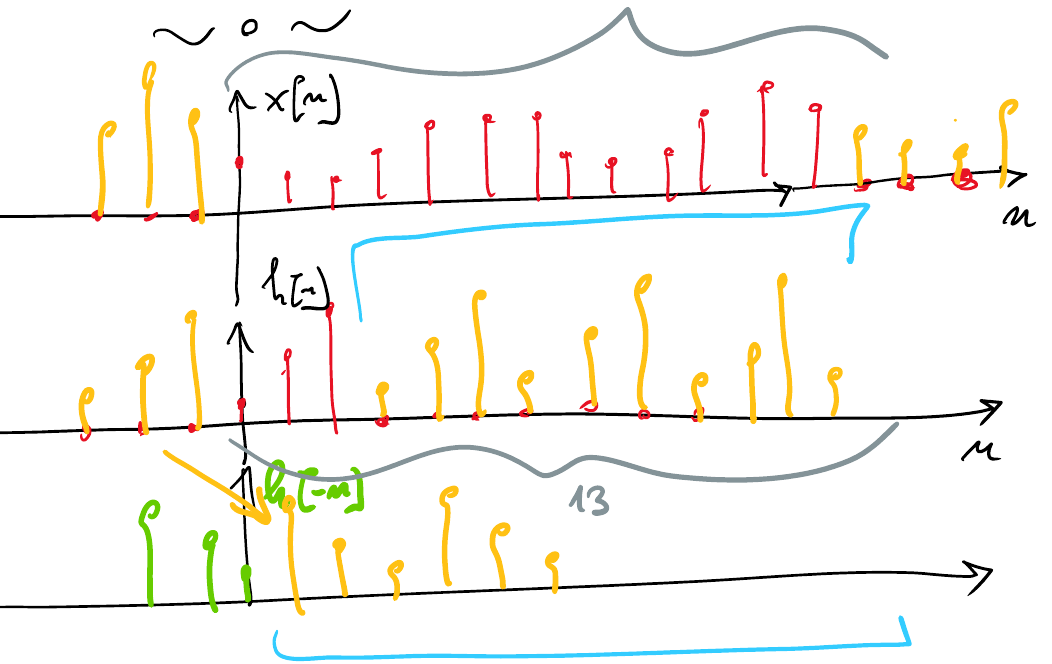
\includegraphics[scale=0.35]{immagini/lez25/convoluzioneDFT.jpg}
\end{figure}

possiamo quindi dare la proprieta' della convoluzione della DFT, se i campioni dei due segnali sono uguali:

\[
x_p[n] * h_p[n] \leftrightarrow  X_{[k]} H_{[k]} \mbox{ SE } M = N
\]

Ma come possiamo rendere $M = N$, i due segnali di lunghezza uguale?
Esiste una tecnica chiamata ZERO PADDING che consiste nel mettere tanti zeri nella sequenza piu' corta.
Dimostriamo che funziona:
\[\begin{split}
    x[n] \leftrightarrow X_{[k]} = \sum_{n=0}^{N-1} x[n] e^{-j \frac{2\pi}{N}kn} \\
    \Tilde{x}[n] = \{x[n]; 0 \mbox{ ... }0\} \leftrightarrow \Tilde{T}_{[k]} = \sum_{n=0}^{2N-1} \Tilde{x}[n] e^{-j \frac{2\pi}{2N}kn} \\
    = \sum_{n=0}^{N-1} x[n] e^{-j \frac{2\pi}{2N}kn} \\
    k = 2h\\
    \mbox{Quando k pari } = \sum_{n=0}^{N-1} x[n] e^{-j \frac{2\pi}{N}hn}
\end{split}\]

Allargando il segnale con tanti zeri abbiamo portato un aumento della visibilita' spettrale, che e' passata da $\frac{2\pi}{N}$ a $\frac{2\pi}{2N}$. Ovvero parlando in termini pratici ho piu' campioni con frequenze piu' vicine tra di loro (griglia di campionamento piu' fine).

Ma per i valori dispari cosa abbiamo ottenuti? Succede che la DFT viene campionata in punti che precedentemente non avevamo. Questa e' una cosa che molto spesso viene ricercata e nel calcolo numerico e' una tecnica spettrale.


\begin{figure}[ht!]
    \centering
    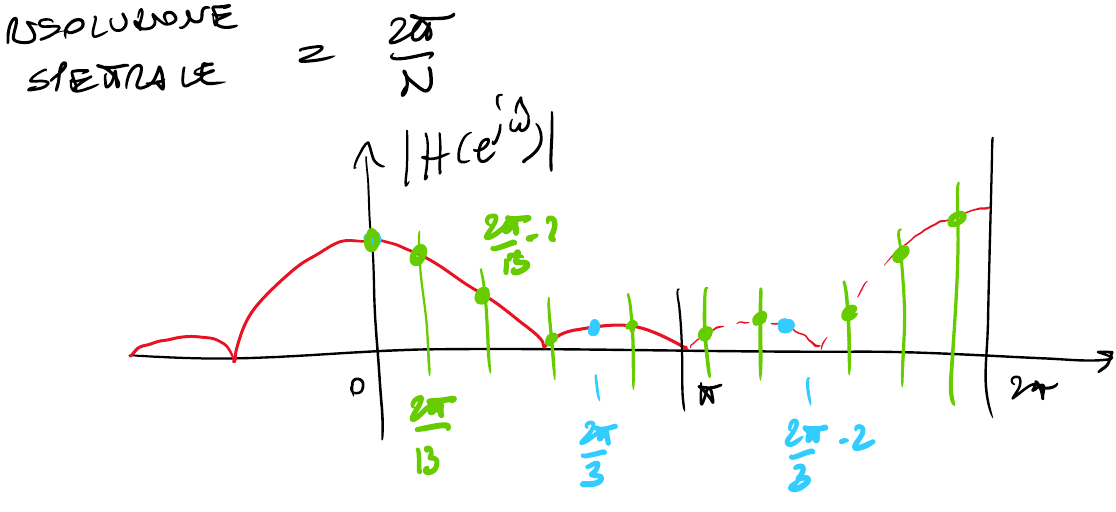
\includegraphics[scale=0.35]{immagini/lez25/aumentoRisoluzioneSpettrale.jpg}
\end{figure}

\section{Riassuno filtraggio LTI}

\begin{figure}[ht!]
    \centering
    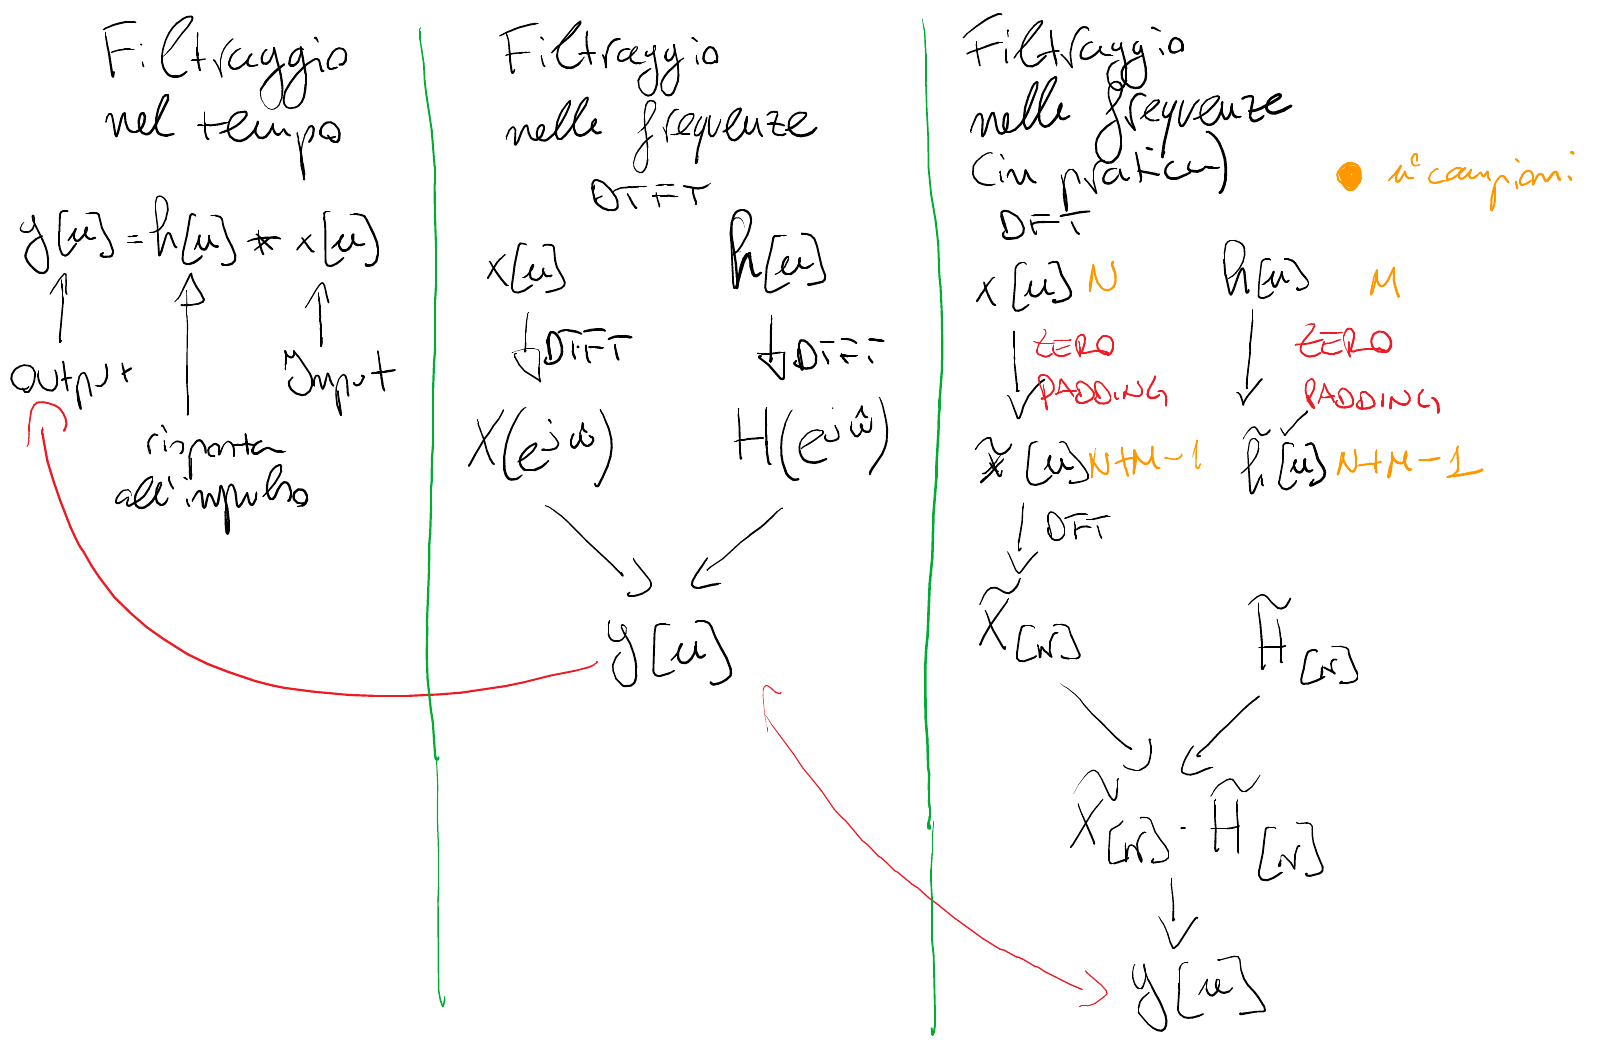
\includegraphics[scale=0.35]{immagini/lez25/filtraggio.jpg}
\end{figure}

Possiamo provare a calcolare il filtraggio utilizzando la DFT e lo zero padding.
Comunque notiamo che il problema delle repliche nelle convoluzione e' presente lo stesso ma abbiamo visto che aggiungendo degli zeri al segnale abbiamo allontanato le repliche spettrali dall'alias principale, quindi l'intuizione e' di aggiungere altri zeri in modo da poter fare una convoluzione "pulita". Ma di quanti zeri ho bisogno? N+M-1 campioni ad entrambi i segnali (non solo il piu' corto).

\begin{figure}[ht!]
    \centering
    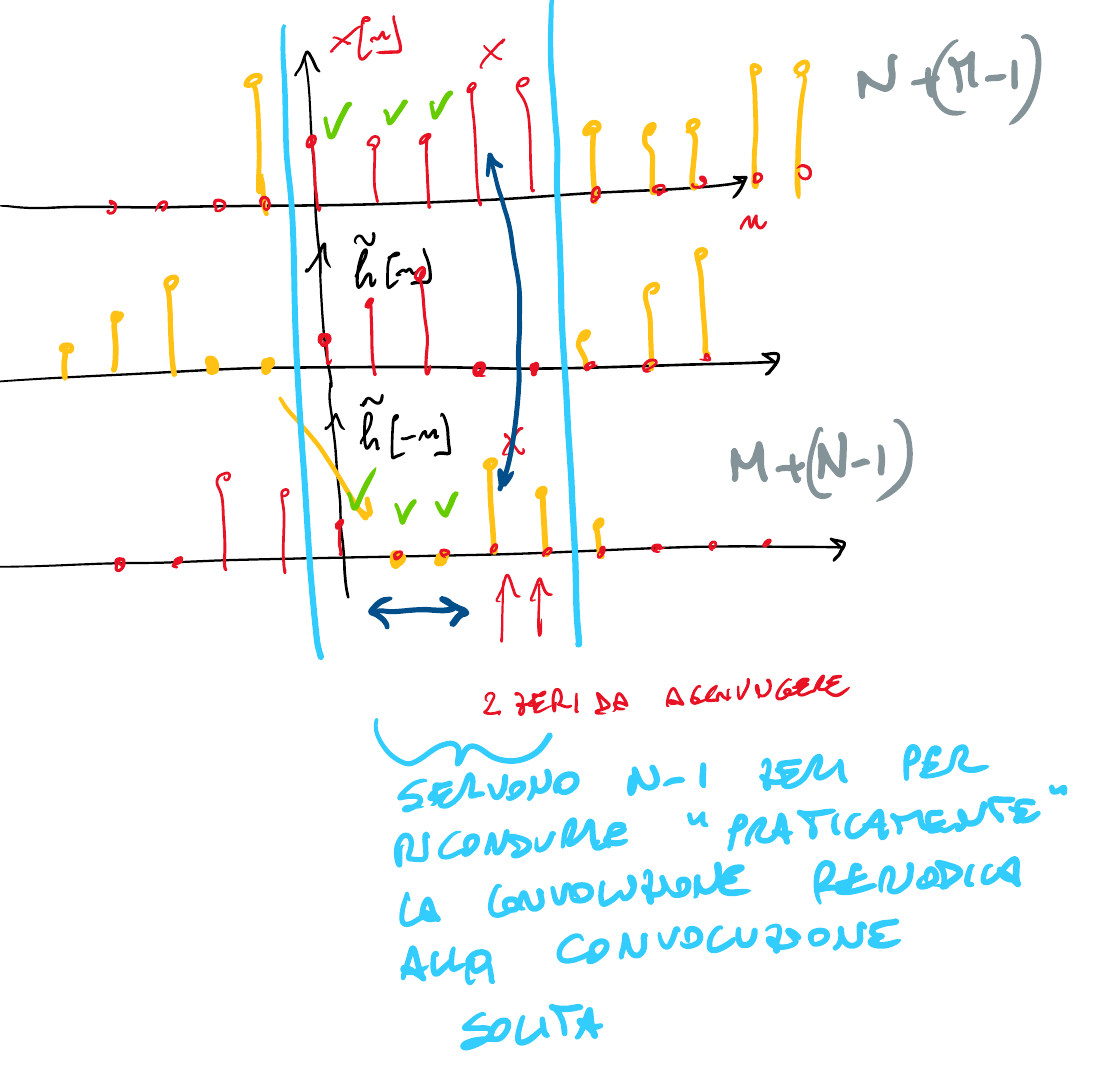
\includegraphics[scale=0.35]{immagini/lez25/convoluzioneZeroPadding.jpg}
\end{figure}

\section{Fast Fourier Trasnsform FFT}

Quello che abbiamo visto con il filtraggio tramite DFT e' computazionalmente molto svantaggioso (e perdente rispetto agli altre due approcci). Ma si sono accorti che la DFT si puo' calcolare semplicemente implementando un algoritmo, tanto semplicemente che a volte e' un'implementazione inclusi direttamente in hardware. 
L'algoritmo per calcolare semplicemente la DFT si chiama Fast Fourier Transform FFT. 
E' un algoritmo che fa parte della famiglia divide et impera, ovvero cerchiamo di dividere il problema in sotto problemi fino ad arrivare ad una "foglia" che e' facilmente risolvibile e successivamente tornare su tramite la ricorsione. Teoricamente e' un algoritmo ricorsivo, ma nella pratica non e' implementato in maniera ricorsiva, perche' e' un implementazione che costa meno.

Vediamo come funziona. Abbiamo una sequenza di campioni che e' lunga una potenza di due $N = 2^M$ (oggi non e' piu' obbligatorio che lo sia, ma e' il caso migliore), l'idea e' di prendere i numeri negli indici pari e metterli in un altro vettore e fare la stessa cosa con i numeri negli indici dispari, ripetere queste istruzioni finche' il vettore e' composto di due elementi. Una volta che ho tanti vettori composti da due elementi siamo arrivati al caso base. Ma perche' e' questo il caso base? Semplicemente perche' per calcolare la DFT di un vettore con due elementi devo fare 0 moltiplicazioni e di conseguenza e' molto poco oneroso computazionalmente.

\begin{figure}[ht!]
    \centering
    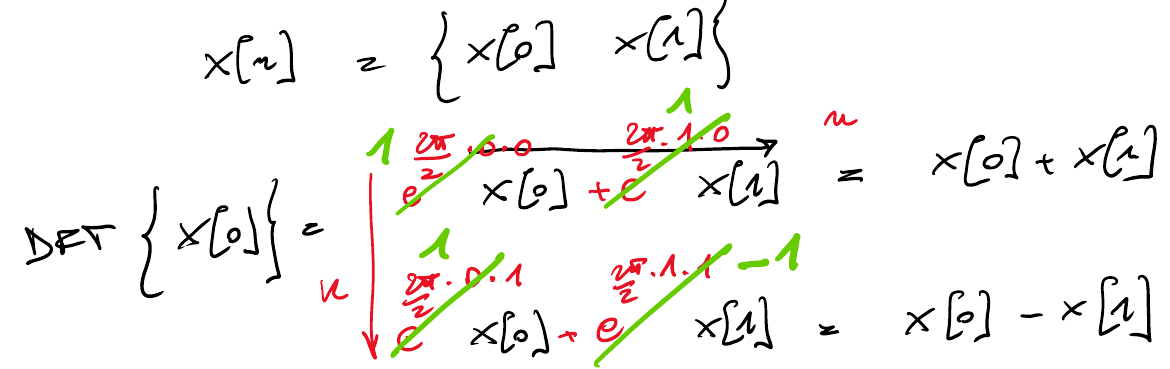
\includegraphics[scale=0.35]{immagini/lez25/DFT2Elementi.jpg}
\end{figure}

A questo punto, dopo aver capito qual'e' il caso base della ricorsione, dobbiamo tornare indietro e ricostruire i vari vettori partendo dal casi base.
Consideriamo una DFT generale di un segnale, ci siamo posti nella condizione in cui $N=2^M$, possiamo spaccare la sommatoria in due, in una consideriamo i numeri pari e nell'altra i numeri dispari:

\[\begin{split}
    X_{[k]} &= \sum_{n=0}^{N-1} x[n] e^{-j \frac{2\pi}{N}\cdot kn} \\
    &= \sum_{l=0}^{\frac{N}{2}-1} x[2l] e^{-j \frac{2\pi}{N}\cdot 2lk} + \sum_{l=0}^{\frac{N}{2}-1} x[2l+1] e^{-j \frac{2\pi}{N}\cdot (2l+1) k}\\
    \mbox{Riscriviamo } e^{-j \frac{2\pi}{N}\cdot (2l+1) k} &= e^{-j \frac{2\pi}{N}\cdot 2l k} e^{-j \frac{2\pi}{N}\cdot k} \\
    &\mbox{Portiamo furi l'esponenziale che non dipende da l} \\
    &= \sum_{l=0}^{\frac{N}{2}-1} x[2l] e^{-j \frac{2\pi}{N}\cdot 2lk} + (e^{-j \frac{2\pi}{N}k}) \sum_{l=0}^{\frac{N}{2}-1} x[2l+1] e^{-j \frac{2\pi}{N}\cdot lk} \\
\end{split}\]

Abbiamo quindi ottenuto una sommatoria dei valori pari piu' una sommatoria dei valori dispari moltiplicata per un fattore che ad ogni iterazione scala (0,1,2 ... N).

Guardiamo adesso una tabella che ci fa capire praticamente quanto e' piu' vantaggiosa la FFT in termini di moltiplicazioni rispetto alle DFT:

\begin{table}[ht!]
    \centering
    \begin{tabular}{c|c|c}
        N & Moltiplicazioni FFT & Moltiplicazioni DFT  \\
        \hline
        2 & 0 & 4 \\
        4 & $2 \cdot 0 + 4 = 4$ & 16 \\
        8 & $2 \cdot 4 + 8 = 16$ & 64 \\
        16 & $2 \cdot 16 + 16 = 44$ & 256 \\
        N & $N(\log_2 N-1)$ & $N^2$ \\
        1000 & $2,8 \cdot 10^4$ & $10^6$ \\
        $10^6$ & $5,8 \cdot 10^7$ & $10^12$ \\
    \end{tabular}
\end{table}

\subsection{Costo computazionale filtraggio nel tempo (convoluzoine) VS frequenza (DFT)}
\begin{figure}[ht!]
    \centering
    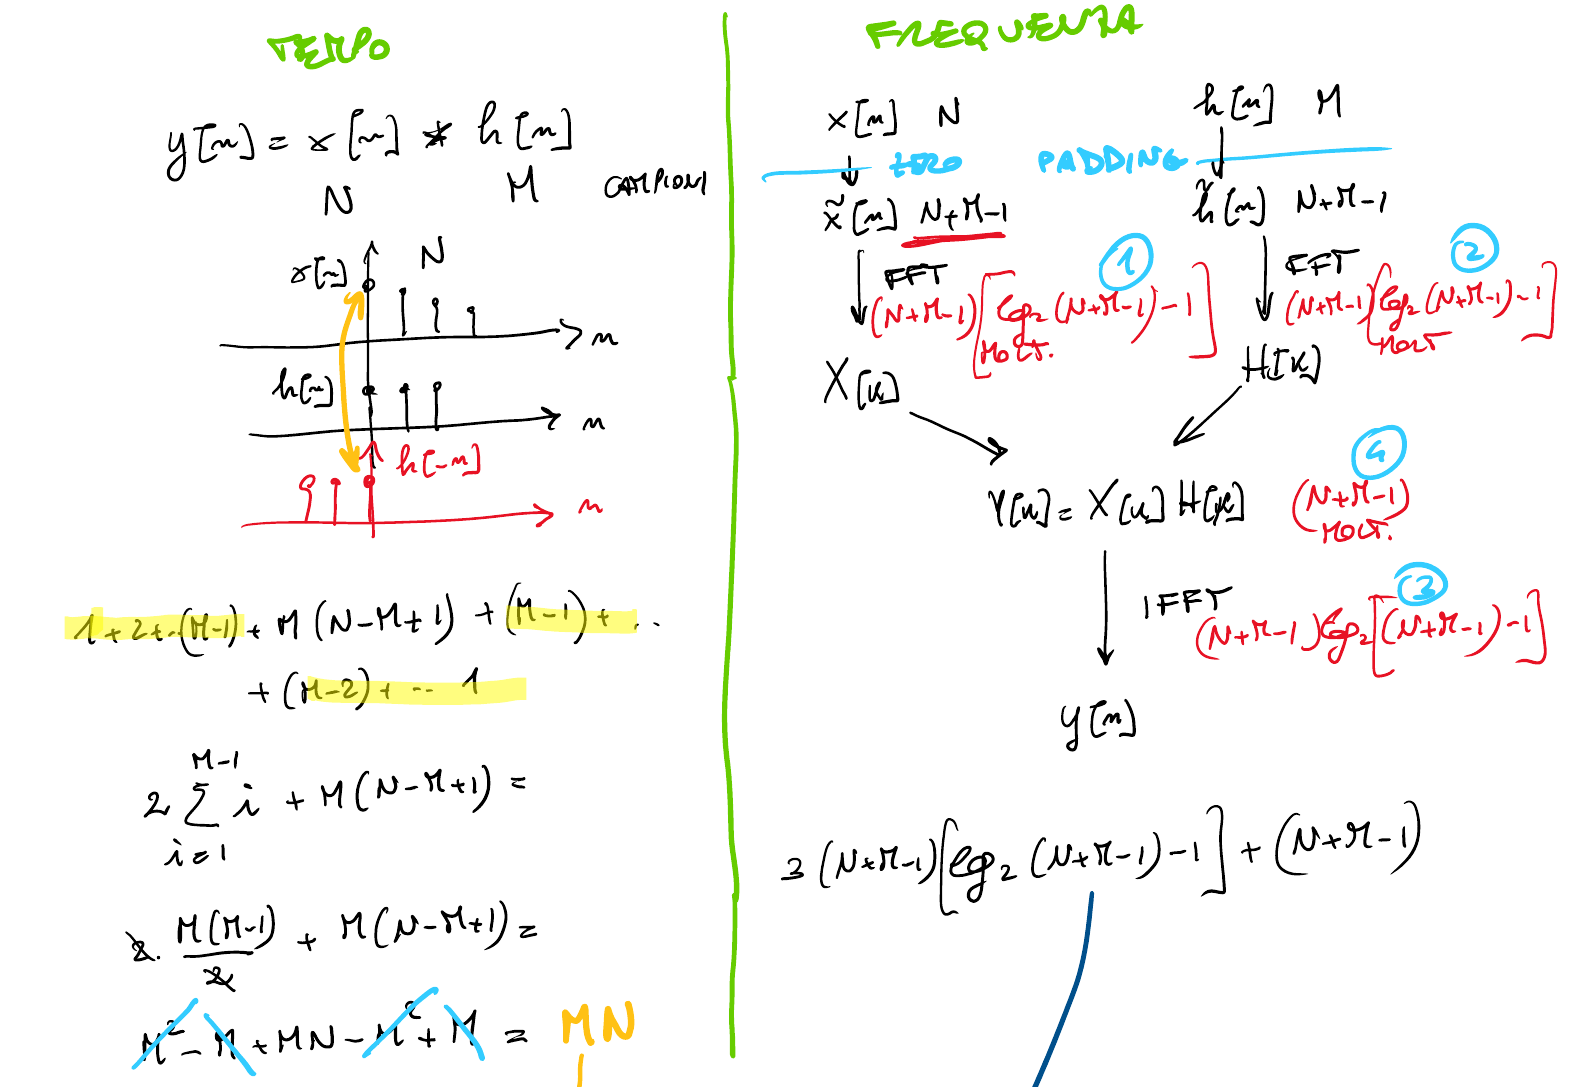
\includegraphics[scale=0.35]{immagini/lez26/convoluzioneTempoFrequenza.jpg}
\end{figure}

\begin{figure}[ht!]
    \centering
    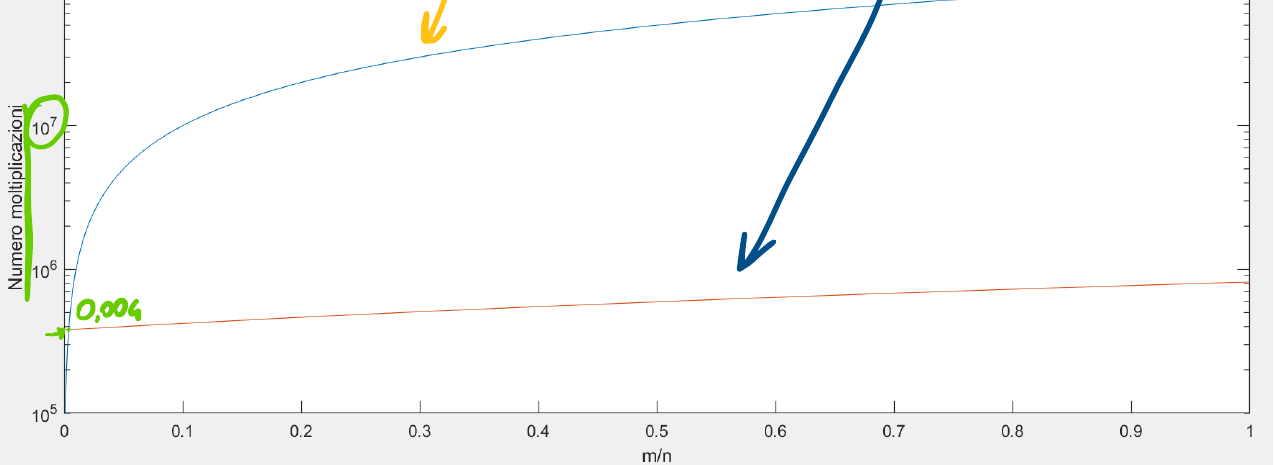
\includegraphics[scale=0.35]{immagini/lez26/graficoCostoFiltraggio.jpg}
\end{figure}

Da questo confronto tiriamo fuori una regola generale se M e' molto minore di N (ovvero il filtro e' corto) bisogna utilizzare il filtraggio nel tempo, viceversa se M e' simile ad N (ovvero il filtro e' lungo quanto il segnale) bisogna usare il filtraggio nelle frequenze, perche' in entrambi i casi sono computazionalmente meno onerosi.

\subsection{Base ortonormale}
Notiamo che a differenza di come avevamo fatto con la serie di Fourier e la DTFT, per la DFT non abbiamo visto una definizione che utilizza il prodotto scalare, questo perche' essendo la DFT un vettore numerabile, il prodotto scalare e' semplicemente il prodotto scalare del vettore per una base ortogonale.

Ma perche' ortogonale e non ortonormale, come invece era per serie di Fourier e DTFT?
Ricordiamo inizialmente che un vettore e' ortogonali quando prodotto scalare per una base e' 0. Dimostriamo quindi che facendo il prodotto vettoriale tra un elemento della DFT ed una base otteniamo 0:

\[\begin{split}
    <e^{j \frac{2\pi}{N}kn}; e^{j \frac{2\pi}{N}hn}> &= \sum_{n=0}^{N-1} e^{j \frac{2\pi}{N}kn} e^{j \frac{2\pi}{N}hn} \\
    &= \sum_{n=0}^{N-1} (e^{j \frac{2\pi}{N}})^{(k-h)n} = \frac{1 - e^{j \frac{2\pi}{N}kn}}{1 - e^{j\frac{2\pi}{N}}(k-h)}\\
    &= 
    \begin{cases}
    \frac{0}{N \neq 0} = 0 \text{ se } h \neq k \\
    N \text{ se } h=k\\
    \end{cases}
\end{split}\]

\subsection{Legge di conservazione (Parseval)}

\begin{equation}
    \sum_{n=0}^{N_1} |x[n]|^2 = \frac{1}{N} \sum_{k=0}^{N-1} |X_{[k]}|^2
\end{equation}

E' l'energia del segnale se il segnale ha supporto compatto, altrimenti se e' periodico e' l'energia nel periodo.